\documentclass[mathserif,usenames,dvipsnames]{beamer}

%\usetheme{LCOM}
\usetheme{Madrid}
\usepackage{hyperref}
\usepackage{listings}
\usepackage{graphicx}
\usepackage[portuguese]{babel}
\usepackage[utf8]{inputenc}
\usepackage[T1]{fontenc}
\usepackage{booktabs}
\usepackage{amsmath,amssymb,amsthm,mathrsfs,amsfonts,dsfont}
\usepackage{adjustbox}
\usepackage{array}
\usepackage{longtable}
\usepackage{psfrag}
\usepackage{caption}
\usepackage{placeins}
\usepackage{subfig}
\usepackage{multirow}
\usepackage[siunitx, american]{circuitikz}
\usetikzlibrary{decorations.markings}
\usetikzlibrary {arrows, positioning}
\usetikzlibrary{plotmarks}

\uselanguage{portuguese}
\languagepath{portuguese}
\deftranslation[to=portuguese]{Theorem}{Teorema}
\deftranslation[to=portuguese]{theorem}{teorema}

\definecolor{green_variavel}{rgb}{0.13,0.57,0.2}
\usecolortheme[named=green_variavel]{structure}

%\definecolor{red_variavel}{rgb}{0.5,0,0}
%\usecolortheme[named=red_variavel]{structure}

\newcommand{\wait}{\vfill}
%\newcommand{\wait}{\pause}

\newcommand*\circled[1]{\tikz[baseline=(char.base)]{
		\node[shape=circle,draw,inner sep=2pt] (char) {#1};}}
	
\DeclareMathAlphabet\mathbfcal{OMS}{cmsy}{b}{n}
\newcommand\blfootnote[1]{%
	\begingroup
	\renewcommand\thefootnote{}\footnote{#1}%
	\addtocounter{footnote}{-1}%
	\endgroup
}

\setbeamertemplate{frametitle continuation}[from second][]

\title[Funções Singulares]{Autotransformador} 
\author[Vinícius Lagrota]{Vinícius Lagrota Rodrigues da Costa}
\institute[CES]{
\includegraphics[width=0.3\textwidth]{figuras/ces}\\[\medskipamount]
	Centro de Ensino Superior de Juiz de Fora}
\date{\today}

\begin{document}

\begin{frame}
\maketitle 
\end{frame}

\begin{frame}
\frametitle{Sumário}
\tableofcontents
\end{frame}

%------------------------------------------------------------------------------------
\section{Recapitulação}
\subsection{Indução mútua}
%------------------------------------------------------------------------------------
%inner square side length
\def\a{3.0}
%outer square side length
\def\b{5.0}
% x displacement of back squares
\def\dx{0.8}
% y displacement of back squares
\def\dy{0.5}
\def\lx{1.0}
\def\ly{1.0}
% round corner correction
\def\dr{0.02}
\def\figScale{0.45}

\begin{frame}
\frametitle{Recapitulação}
\framesubtitle{Indução mútua}
	
	\begin{overprint}
		\only<1>
		{	
			\begin{block}{Conceito}
				\begin{itemize}
					\item Uma corrente variante circulando na bobina 1 gera um fluxo magnético que também enlaça a bobina 2 e gera nesta uma tensão.
					\item O inverso também é verdadeiro.
					\item Fenômeno conhecido como \textbf{indução mútua}.
					\item A tensão induzida é proporcional à taxa de variação do fluxo magnético.
				\end{itemize}
			\end{block}
			\begin{center}
				\begin{circuitikz}[scale = \figScale, global scale/.style={scale=1.0}, rotate=-5, xslant=-0.1, thick, every node/.style={transform shape, scale=0.8}, decoration={markings, mark=at position 0.5 with {\arrow{latex}}}]
					\begin{scope}[even odd rule]
						\filldraw[rounded corners=2pt, fill=gray, rotate=-0, opacity=1.0] (\dx,
						\dy) rectangle ++(5,5) (\lx+\dx,\ly+\dy) rectangle ++(\a, \a);
						\fill [rounded corners=2pt, fill=gray] (\b, 0) --++ (0, \dy+\dr+0.02) --++(\dx, 0) --cycle;
						\fill [rounded corners=2pt, fill=gray] (0, \b) --++ (\dx+\dr+0.02, 0) --++(0, \dy)--cycle;
						\filldraw[rounded corners=2pt, fill=gray!50, rotate=-0] (0,0) rectangle
						++(\b, \b) (\lx,\ly) rectangle ++(\a, \a);
						\draw (\b-\dr,\dr) --++(\dx, \dy);
						\draw (\b-\dr,\b-\dr) --++(\dx, \dy);
						\draw (\dr,\b-\dr) --++(\dx, \dy);
						\draw [blue, thick, postaction={decorate}] (0, \ly) --++(-1.5,0);
						\foreach \z in {0,.24,.48,...,2.5}
						{
							\draw [rounded corners=2pt,blue, thick]
							(-0.0,\ly+\z+0.08)--(-0.09,\ly+\z) -- (\lx, \ly+\z)--++(0.89,0.5)
							--++(-0.08, 0.05);
						}
						\draw [rounded corners=2pt,blue, thick, postaction={decorate}] (-1.5,
						\ly+2.8) --++(1.5,0) node[black, above, pos=0.4] {\Huge $i_1$};
						
						
						\draw[-latex] (-\lx, \ly+0.2) --++ (0, 2.4) node[midway, left] {\Huge $v_1$};
									
						\draw [rounded corners=2pt,red, thick] (\a+\lx-2*\dr,
						\ly+2*\dr)--++(-\dr, -\dr)--++(\lx+\dx+2*\dr, 0);
						\draw [red, postaction={decorate}] (\b+\dx-\dr, \ly+\dr)--++(\a/2, 0);
						
						
		%				\draw [rounded corners=2pt, red, thick, postaction={decorate}]
		%				(\a+3*\lx-0.2, \ly+3.1) --++(\a/2, 0) node[black, midway, above] {\Huge $i_2$};
		
		
						\draw [rounded corners=2pt, red, thick, postaction={decorate}]
						(7.3, 4.1) --++ (-1.5, 0) node[black, midway, above] {\Huge $i_2$};
						
						
						
						
						\foreach \z in {.125,.25,.375,...,2.5}
						{
							\draw [rounded corners=2pt, red, thick] (\a+\lx,\ly+\z+0.1)--
							(\a+\lx-0.07,\ly+\z) -- (\a+2*\lx, \ly+\z)--++(0.87,0.5)--++(-0.06,
							0.06);
						}
						\draw[-latex] (2*\a+\lx, \ly+0.2) --++(0, 2.7) node[midway, right] {\Huge $v_2$};
						
						%end
						\draw (0.5, 0.5) node[] {\Huge $\circled{1}$};
						\draw (4.5, 0.5) node[] {\Huge $\circled{2}$};
						
						\draw [-latex, rounded corners=2pt, blue, thick]
						(1, 0.5) --++ (1, 0) node[black, right] {\Huge $\textcolor{blue}{\phi_1}$};
						
						\draw [-latex, rounded corners=2pt, red, thick]
						(4, 4.5) --++ (-1, 0) node[black, left] {\Huge $\textcolor{red}{\phi_2}$};
					\end{scope}
				\end{circuitikz}
			\end{center}
		}
		\only<2>
		{
			\begin{center}
				\begin{circuitikz}[scale = \figScale, global scale/.style={scale=1.0}, rotate=-5, xslant=-0.1, thick, every node/.style={transform shape, scale=0.8}, decoration={markings, mark=at position 0.5 with {\arrow{latex}}}]
					\begin{scope}[even odd rule]
						\filldraw[rounded corners=2pt, fill=gray, rotate=-0, opacity=1.0] (\dx,
						\dy) rectangle ++(5,5) (\lx+\dx,\ly+\dy) rectangle ++(\a, \a);
						\fill [rounded corners=2pt, fill=gray] (\b, 0) --++ (0, \dy+\dr+0.02) --++(\dx, 0) --cycle;
						\fill [rounded corners=2pt, fill=gray] (0, \b) --++ (\dx+\dr+0.02, 0) --++(0, \dy)--cycle;
						\filldraw[rounded corners=2pt, fill=gray!50, rotate=-0] (0,0) rectangle
						++(\b, \b) (\lx,\ly) rectangle ++(\a, \a);
						\draw (\b-\dr,\dr) --++(\dx, \dy);
						\draw (\b-\dr,\b-\dr) --++(\dx, \dy);
						\draw (\dr,\b-\dr) --++(\dx, \dy);
						\draw [blue, thick, postaction={decorate}] (0, \ly) --++(-1.5,0);
						\foreach \z in {0,.24,.48,...,2.5}
						{
							\draw [rounded corners=2pt,blue, thick]
							(-0.0,\ly+\z+0.08)--(-0.09,\ly+\z) -- (\lx, \ly+\z)--++(0.89,0.5)
							--++(-0.08, 0.05);
						}
						\draw [rounded corners=2pt,blue, thick, postaction={decorate}] (-1.5,
						\ly+2.8) --++(1.5,0) node[black, above, pos=0.4] {\Huge $i_1$};
						
						
						\draw[-latex] (-\lx, \ly+0.2) --++ (0, 2.4) node[midway, left] {\Huge $v_1$};
						
						\draw [rounded corners=2pt,red, thick] (\a+\lx-2*\dr,
						\ly+2*\dr)--++(-\dr, -\dr)--++(\lx+\dx+2*\dr, 0);
						\draw [red, postaction={decorate}] (\b+\dx-\dr, \ly+\dr)--++(\a/2, 0);
						
						
						%				\draw [rounded corners=2pt, red, thick, postaction={decorate}]
						%				(\a+3*\lx-0.2, \ly+3.1) --++(\a/2, 0) node[black, midway, above] {\Huge $i_2$};
						
						
						\draw [rounded corners=2pt, red, thick, postaction={decorate}]
						(7.3, 4.1) --++ (-1.5, 0) node[black, midway, above] {\Huge $i_2$};
						
						
						
						
						\foreach \z in {.125,.25,.375,...,2.5}
						{
							\draw [rounded corners=2pt, red, thick] (\a+\lx,\ly+\z+0.1)--
							(\a+\lx-0.07,\ly+\z) -- (\a+2*\lx, \ly+\z)--++(0.87,0.5)--++(-0.06,
							0.06);
						}
						\draw[-latex] (2*\a+\lx, \ly+0.2) --++(0, 2.7) node[midway, right] {\Huge $v_2$};
						
						%end
						\draw (0.5, 0.5) node[] {\Huge $\circled{1}$};
						\draw (4.5, 0.5) node[] {\Huge $\circled{2}$};
						
						\draw [-latex, rounded corners=2pt, blue, thick]
						(1, 0.5) --++ (1, 0) node[black, right] {\Huge $\textcolor{blue}{\phi_1}$};
						
						\draw [-latex, rounded corners=2pt, red, thick]
						(4, 4.5) --++ (-1, 0) node[black, left] {\Huge $\textcolor{red}{\phi_2}$};
					\end{scope}
				\end{circuitikz}
			\end{center}	
			\begin{block}{Conceito}
				\begin{itemize}
					\item Os fluxos produzidos ($\phi_1$ e $\phi_2$) estão ambos no sentido anti-horário $\Rightarrow$ acoplamento mútuo tende a aumentar a aumentar a intensidade das tensões induzidas. 
%					\item Os fluxos magnéticos são completamente compreendidos definidos pelas correntes $i_1$ e $i_2$ variáveis no tempo.
				\end{itemize}
			\end{block}
		}
%		\only<3>
%		{
%			\begin{center}
%				\begin{circuitikz}[scale = \figScale, global scale/.style={scale=1.0}, rotate=-5, xslant=-0.1, thick, every node/.style={transform shape, scale=0.8}, decoration={markings, mark=at position 0.5 with {\arrow{latex}}}]
%					\begin{scope}[even odd rule]
%						\filldraw[rounded corners=2pt, fill=gray, rotate=-0, opacity=1.0] (\dx,
%						\dy) rectangle ++(5,5) (\lx+\dx,\ly+\dy) rectangle ++(\a, \a);
%						\fill [rounded corners=2pt, fill=gray] (\b, 0) --++ (0, \dy+\dr+0.02) --++(\dx, 0) --cycle;
%						\fill [rounded corners=2pt, fill=gray] (0, \b) --++ (\dx+\dr+0.02, 0) --++(0, \dy)--cycle;
%						\filldraw[rounded corners=2pt, fill=gray!50, rotate=-0] (0,0) rectangle
%						++(\b, \b) (\lx,\ly) rectangle ++(\a, \a);
%						\draw (\b-\dr,\dr) --++(\dx, \dy);
%						\draw (\b-\dr,\b-\dr) --++(\dx, \dy);
%						\draw (\dr,\b-\dr) --++(\dx, \dy);
%						\draw [blue, thick, postaction={decorate}] (0, \ly) --++(-1.5,0);
%						\foreach \z in {0,.24,.48,...,2.5}
%						{
%							\draw [rounded corners=2pt,blue, thick]
%							(-0.0,\ly+\z+0.08)--(-0.09,\ly+\z) -- (\lx, \ly+\z)--++(0.89,0.5)
%							--++(-0.08, 0.05);
%						}
%						\draw [rounded corners=2pt,blue, thick, postaction={decorate}] (-1.5,
%						\ly+2.8) --++(1.5,0) node[black, above, pos=0.4] {\Huge $i_1$};
%						
%						
%						\draw[-latex] (-\lx, \ly+0.2) --++ (0, 2.4) node[midway, left] {\Huge $v_1$};
%						
%						\draw [rounded corners=2pt,red, thick] (\a+\lx-2*\dr,
%						\ly+2*\dr)--++(-\dr, -\dr)--++(\lx+\dx+2*\dr, 0);
%						\draw [red, postaction={decorate}] (\b+\dx-\dr, \ly+\dr)--++(\a/2, 0);
%						
%						
%						%				\draw [rounded corners=2pt, red, thick, postaction={decorate}]
%						%				(\a+3*\lx-0.2, \ly+3.1) --++(\a/2, 0) node[black, midway, above] {\Huge $i_2$};
%						
%						
%						\draw [rounded corners=2pt, red, thick, postaction={decorate}]
%						(7.3, 4.1) --++ (-1.5, 0) node[black, midway, above] {\Huge $i_2$};
%						
%						
%						
%						
%						\foreach \z in {.125,.25,.375,...,2.5}
%						{
%							\draw [rounded corners=2pt, red, thick] (\a+\lx,\ly+\z+0.1)--
%							(\a+\lx-0.07,\ly+\z) -- (\a+2*\lx, \ly+\z)--++(0.87,0.5)--++(-0.06,
%							0.06);
%						}
%						\draw[-latex] (2*\a+\lx, \ly+0.2) --++(0, 2.7) node[midway, right] {\Huge $v_2$};
%						
%						%end
%						\draw (0.5, 0.5) node[] {\Huge $\circled{1}$};
%						\draw (4.5, 0.5) node[] {\Huge $\circled{2}$};
%						
%						\draw [-latex, rounded corners=2pt, blue, thick]
%						(1, 0.5) --++ (1, 0) node[black, right] {\Huge $\textcolor{blue}{\phi_1}$};
%						
%						\draw [-latex, rounded corners=2pt, red, thick]
%						(4, 4.5) --++ (-1, 0) node[black, left] {\Huge $\textcolor{red}{\phi_2}$};
%					\end{scope}
%				\end{circuitikz}
%			\end{center}	
%			\begin{block}{Conceito}
%				Portanto,
%				\begin{equation}\label{key}
%					\left\{ \begin{array}{l}
%					\frac{{\partial {\phi _1}}}{{\partial {i_1}}}d{i_1} + \frac{{\partial {\phi _1}}}{{\partial {i_2}}}d{i_2} = d{\phi _1}\\[5pt]
%					\frac{{\partial {\phi _2}}}{{\partial {i_1}}}d{i_1} + \frac{{\partial {\phi _2}}}{{\partial {i_2}}}d{i_2} = d{\phi _2}
%					\end{array} \right.
%				\end{equation}
%				\begin{equation}\label{key}
%				\left\{ \begin{array}{l}
%				\left( {{N_1}\frac{{\partial {\phi _1}}}{{\partial {i_1}}}} \right)\frac{{d{i_1}}}{{dt}} + \left( {{N_1}\frac{{\partial {\phi _1}}}{{\partial {i_2}}}} \right)\frac{{d{i_2}}}{{dt}} = {N_1}\frac{{d{\phi _1}}}{{dt}}\\[5pt]
%				\left( {{N_2}\frac{{\partial {\phi _2}}}{{\partial {i_1}}}} \right)\frac{{d{i_1}}}{{dt}} + \left( {{N_2}\frac{{\partial {\phi _2}}}{{\partial {i_2}}}} \right)\frac{{d{i_2}}}{{dt}} = {N_2}\frac{{d{\phi _2}}}{{dt}}
%				\end{array} \right.
%				\end{equation}
%			\end{block}
%		}
%		\only<4>
%		{
%			\begin{center}
%				\begin{circuitikz}[scale = \figScale, global scale/.style={scale=1.0}, rotate=-5, xslant=-0.1, thick, every node/.style={transform shape, scale=0.8}, decoration={markings, mark=at position 0.5 with {\arrow{latex}}}]
%					\begin{scope}[even odd rule]
%						\filldraw[rounded corners=2pt, fill=gray, rotate=-0, opacity=1.0] (\dx,
%						\dy) rectangle ++(5,5) (\lx+\dx,\ly+\dy) rectangle ++(\a, \a);
%						\fill [rounded corners=2pt, fill=gray] (\b, 0) --++ (0, \dy+\dr+0.02) --++(\dx, 0) --cycle;
%						\fill [rounded corners=2pt, fill=gray] (0, \b) --++ (\dx+\dr+0.02, 0) --++(0, \dy)--cycle;
%						\filldraw[rounded corners=2pt, fill=gray!50, rotate=-0] (0,0) rectangle
%						++(\b, \b) (\lx,\ly) rectangle ++(\a, \a);
%						\draw (\b-\dr,\dr) --++(\dx, \dy);
%						\draw (\b-\dr,\b-\dr) --++(\dx, \dy);
%						\draw (\dr,\b-\dr) --++(\dx, \dy);
%						\draw [blue, thick, postaction={decorate}] (0, \ly) --++(-1.5,0);
%						\foreach \z in {0,.24,.48,...,2.5}
%						{
%							\draw [rounded corners=2pt,blue, thick]
%							(-0.0,\ly+\z+0.08)--(-0.09,\ly+\z) -- (\lx, \ly+\z)--++(0.89,0.5)
%							--++(-0.08, 0.05);
%						}
%						\draw [rounded corners=2pt,blue, thick, postaction={decorate}] (-1.5,
%						\ly+2.8) --++(1.5,0) node[black, above, pos=0.4] {\Huge $i_1$};
%						
%						
%						\draw[-latex] (-\lx, \ly+0.2) --++ (0, 2.4) node[midway, left] {\Huge $v_1$};
%						
%						\draw [rounded corners=2pt,red, thick] (\a+\lx-2*\dr,
%						\ly+2*\dr)--++(-\dr, -\dr)--++(\lx+\dx+2*\dr, 0);
%						\draw [red, postaction={decorate}] (\b+\dx-\dr, \ly+\dr)--++(\a/2, 0);
%						
%						
%						%				\draw [rounded corners=2pt, red, thick, postaction={decorate}]
%						%				(\a+3*\lx-0.2, \ly+3.1) --++(\a/2, 0) node[black, midway, above] {\Huge $i_2$};
%						
%						
%						\draw [rounded corners=2pt, red, thick, postaction={decorate}]
%						(7.3, 4.1) --++ (-1.5, 0) node[black, midway, above] {\Huge $i_2$};
%						
%						
%						
%						
%						\foreach \z in {.125,.25,.375,...,2.5}
%						{
%							\draw [rounded corners=2pt, red, thick] (\a+\lx,\ly+\z+0.1)--
%							(\a+\lx-0.07,\ly+\z) -- (\a+2*\lx, \ly+\z)--++(0.87,0.5)--++(-0.06,
%							0.06);
%						}
%						\draw[-latex] (2*\a+\lx, \ly+0.2) --++(0, 2.7) node[midway, right] {\Huge $v_2$};
%						
%						%end
%						\draw (0.5, 0.5) node[] {\Huge $\circled{1}$};
%						\draw (4.5, 0.5) node[] {\Huge $\circled{2}$};
%						
%						\draw [-latex, rounded corners=2pt, blue, thick]
%						(1, 0.5) --++ (1, 0) node[black, right] {\Huge $\textcolor{blue}{\phi_1}$};
%						
%						\draw [-latex, rounded corners=2pt, red, thick]
%						(4, 4.5) --++ (-1, 0) node[black, left] {\Huge $\textcolor{red}{\phi_2}$};
%					\end{scope}
%				\end{circuitikz}
%			\end{center}	
%			\begin{block}{Conceito}	
%				\begin{equation}\label{key} \tag{2}
%				\left\{ \begin{array}{l}
%				\left( {{N_1}\frac{{\partial {\phi _1}}}{{\partial {i_1}}}} \right)\frac{{d{i_1}}}{{dt}} + \left( {{N_1}\frac{{\partial {\phi _1}}}{{\partial {i_2}}}} \right)\frac{{d{i_2}}}{{dt}} = {N_1}\frac{{d{\phi _1}}}{{dt}}\\[5pt]
%				\left( {{N_2}\frac{{\partial {\phi _2}}}{{\partial {i_1}}}} \right)\frac{{d{i_1}}}{{dt}} + \left( {{N_2}\frac{{\partial {\phi _2}}}{{\partial {i_2}}}} \right)\frac{{d{i_2}}}{{dt}} = {N_2}\frac{{d{\phi _2}}}{{dt}}
%				\end{array} \right.
%				\end{equation}
%				\begin{equation}\label{key} \tag{3}
%				\left\{ \begin{array}{l}
%				{L_1}\frac{{d{i_1}}}{{dt}} + M\frac{{d{i_2}}}{{dt}} = {v_1}\\[5pt]
%				M\frac{{d{i_1}}}{{dt}} + {L_2}\frac{{d{i_2}}}{{dt}} = {v_2}
%				\end{array} \right.
%				\end{equation}
%			\end{block}
%		}
		\only<3>
		{
			\begin{center}
				\begin{circuitikz}[scale = \figScale, global scale/.style={scale=1.0}, rotate=-5, xslant=-0.1, thick, every node/.style={transform shape, scale=0.8}, decoration={markings, mark=at position 0.5 with {\arrow{latex}}}]
					\begin{scope}[even odd rule]
						\filldraw[rounded corners=2pt, fill=gray, rotate=-0, opacity=1.0] (\dx,
						\dy) rectangle ++(5,5) (\lx+\dx,\ly+\dy) rectangle ++(\a, \a);
						\fill [rounded corners=2pt, fill=gray] (\b, 0) --++ (0, \dy+\dr+0.02) --++(\dx, 0) --cycle;
						\fill [rounded corners=2pt, fill=gray] (0, \b) --++ (\dx+\dr+0.02, 0) --++(0, \dy)--cycle;
						\filldraw[rounded corners=2pt, fill=gray!50, rotate=-0] (0,0) rectangle
						++(\b, \b) (\lx,\ly) rectangle ++(\a, \a);
						\draw (\b-\dr,\dr) --++(\dx, \dy);
						\draw (\b-\dr,\b-\dr) --++(\dx, \dy);
						\draw (\dr,\b-\dr) --++(\dx, \dy);
						\draw [blue, thick, postaction={decorate}] (0, \ly) --++(-1.5,0);
						\foreach \z in {0,.24,.48,...,2.5}
						{
							\draw [rounded corners=2pt,blue, thick]
							(-0.0,\ly+\z+0.08)--(-0.09,\ly+\z) -- (\lx, \ly+\z)--++(0.89,0.5)
							--++(-0.08, 0.05);
						}
						\draw [rounded corners=2pt,blue, thick, postaction={decorate}] (-1.5,
						\ly+2.8) --++(1.5,0) node[black, above, pos=0.4] {\Huge $i_1$};
						
						
						\draw[-latex] (-\lx, \ly+0.2) --++ (0, 2.4) node[midway, left] {\Huge $v_1$};
						
						\draw [rounded corners=2pt,red, thick] (\a+\lx-2*\dr,
						\ly+2*\dr)--++(-\dr, -\dr)--++(\lx+\dx+2*\dr, 0);
						\draw [red, postaction={decorate}] (\b+\dx-\dr, \ly+\dr)--++(\a/2, 0);
						
						
						%				\draw [rounded corners=2pt, red, thick, postaction={decorate}]
						%				(\a+3*\lx-0.2, \ly+3.1) --++(\a/2, 0) node[black, midway, above] {\Huge $i_2$};
						
						
						\draw [rounded corners=2pt, red, thick, postaction={decorate}]
						(7.3, 4.1) --++ (-1.5, 0) node[black, midway, above] {\Huge $i_2$};
						
						
						
						
						\foreach \z in {.125,.25,.375,...,2.5}
						{
							\draw [rounded corners=2pt, red, thick] (\a+\lx,\ly+\z+0.1)--
							(\a+\lx-0.07,\ly+\z) -- (\a+2*\lx, \ly+\z)--++(0.87,0.5)--++(-0.06,
							0.06);
						}
						\draw[-latex] (2*\a+\lx, \ly+0.2) --++(0, 2.7) node[midway, right] {\Huge $v_2$};
						
						%end
						\draw (0.5, 0.5) node[] {\Huge $\circled{1}$};
						\draw (4.5, 0.5) node[] {\Huge $\circled{2}$};
						
						\draw [-latex, rounded corners=2pt, blue, thick]
						(1, 0.5) --++ (1, 0) node[black, right] {\Huge $\textcolor{blue}{\phi_1}$};
						
						\draw [-latex, rounded corners=2pt, red, thick]
						(4, 4.5) --++ (-1, 0) node[black, left] {\Huge $\textcolor{red}{\phi_2}$};
					\end{scope}
				\end{circuitikz}
			\end{center}	
			\begin{block}{Conceito}					
				\begin{equation}\label{key} \tag{3}
				\left\{ \begin{array}{l}
				{L_1}\frac{{d{i_1}}}{{dt}} + M\frac{{d{i_2}}}{{dt}} = {v_1}\\[5pt]
				M\frac{{d{i_1}}}{{dt}} + {L_2}\frac{{d{i_2}}}{{dt}} = {v_2}
				\end{array} \right.
				\end{equation}
				Na qual $L_1$ e $L_2$ são as indutâncias próprias das bobinas 1 e 2 e $M$ é a indutância mútua. Note que: 
				\vspace{-0.35cm}
				\begin{equation}\label{key} \tag{4}
				M = {N_1}\frac{{\partial {\phi _1}}}{{\partial {i_2}}} = {N_2}\frac{{\partial {\phi _2}}}{{\partial {i_1}}}
				\end{equation}
			\end{block}
		}
	\end{overprint}
\end{frame}

%------------------------------------------------
\subsection{Notação do ponto}
\begin{frame}
\frametitle{Sumário}
\small
\tableofcontents[currentsubsection]
\end{frame}
%------------------------------------------------
\begin{frame}
\frametitle{Recapitulação}
\framesubtitle{Notação do ponto}
\begin{overprint}
	\only<1>
	{
		\begin{block}{Notação do ponto}
			\begin{itemize}
				\item Utilizado para determinar se as indutâncias próprias e mútuas são somadas ou subtraídas.
				\item Não é conveniente mostrar essas direções em circuitos elétricos $\Rightarrow$ utiliza-se a \textbf{notação do ponto}.
			\end{itemize}
		\end{block}
		\begin{center}
			\begin{circuitikz}[scale = \figScale, global scale/.style={scale=1.0}, rotate=-5, xslant=-0.1, thick, every node/.style={transform shape, scale=0.8}, decoration={markings, mark=at position 0.5 with {\arrow{latex}}}]
				\begin{scope}[even odd rule]
					\filldraw[rounded corners=2pt, fill=gray, rotate=-0, opacity=1.0] (\dx,
					\dy) rectangle ++(5,5) (\lx+\dx,\ly+\dy) rectangle ++(\a, \a);
					\fill [rounded corners=2pt, fill=gray] (\b, 0) --++ (0, \dy+\dr+0.02) --++(\dx, 0) --cycle;
					\fill [rounded corners=2pt, fill=gray] (0, \b) --++ (\dx+\dr+0.02, 0) --++(0, \dy)--cycle;
					\filldraw[rounded corners=2pt, fill=gray!50, rotate=-0] (0,0) rectangle
					++(\b, \b) (\lx,\ly) rectangle ++(\a, \a);
					\draw (\b-\dr,\dr) --++(\dx, \dy);
					\draw (\b-\dr,\b-\dr) --++(\dx, \dy);
					\draw (\dr,\b-\dr) --++(\dx, \dy);
					\draw [blue, thick, postaction={decorate}] (0, \ly) --++(-1.5,0);
					\foreach \z in {0,.24,.48,...,2.5}
					{
						\draw [rounded corners=2pt,blue, thick]
						(-0.0,\ly+\z+0.08)--(-0.09,\ly+\z) -- (\lx, \ly+\z)--++(0.89,0.5)
						--++(-0.08, 0.05);
					}
					\draw [rounded corners=2pt,blue, thick, postaction={decorate}] (-1.5,
					\ly+2.8) --++(1.5,0) node[black, above, pos=0.1] {\Huge $i_1$};
					
					
					\draw[-latex] (-\lx, \ly+0.2) --++ (0, 2.4) node[midway, left] {\Huge $v_1$};
					
					\draw [rounded corners=2pt,red, thick] (\a+\lx-2*\dr,
					\ly+2*\dr)--++(-\dr, -\dr)--++(\lx+\dx+2*\dr, 0);
					\draw [red, postaction={decorate}] (\b+\dx-\dr, \ly+\dr)--++(\a/2, 0);
					
					
					%				\draw [rounded corners=2pt, red, thick, postaction={decorate}]
					%				(\a+3*\lx-0.2, \ly+3.1) --++(\a/2, 0) node[black, midway, above] {\Huge $i_2$};
					
					
					\draw [rounded corners=2pt, red, thick, postaction={decorate}]
					(7.3, 4.1) --++ (-1.5, 0) node[black, midway, above, pos=0.1] {\Huge $i_2$};
					
					
					
					
					\foreach \z in {.125,.25,.375,...,2.5}
					{
						\draw [rounded corners=2pt, red, thick] (\a+\lx,\ly+\z+0.1)--
						(\a+\lx-0.07,\ly+\z) -- (\a+2*\lx, \ly+\z)--++(0.87,0.5)--++(-0.06,
						0.06);
					}
					\draw[-latex] (2*\a+\lx, \ly+0.2) --++(0, 2.7) node[midway, right] {\Huge $v_2$};
					
					%end
					\draw (0.5, 0.5) node[] {\Huge $\circled{1}$};
					\draw (4.5, 0.5) node[] {\Huge $\circled{2}$};
					
					\draw [-latex, rounded corners=2pt, blue, thick]
					(1, 0.5) --++ (1, 0) node[black, right] {\Huge $\textcolor{blue}{\phi_1}$};
					
					\draw [-latex, rounded corners=2pt, red, thick]
					(4, 4.5) --++ (-1, 0) node[black, left] {\Huge $\textcolor{red}{\phi_2}$};
					
					\node[mark size=5pt,color=blue] at (-0.5,4.25) {\pgfuseplotmark{*}};
					\node[mark size=5pt,color=red] at (6.25,4.5) {\pgfuseplotmark{*}};
				\end{scope}
			\end{circuitikz}
		\end{center}
	}
	\only<2>
	{
		\vspace{-0.3cm}
		\begin{center}
			Correntes entram no ponto $\Rightarrow$ Fluxo magnéticos somadas.
		\end{center}
		\vspace{-0.3cm}
		\begin{minipage}[b]{0.4\linewidth}
			\begin{center}
				\begin{circuitikz}[scale = \figScale, global scale/.style={scale=1.0}, rotate=-5, xslant=-0.1, thick, every node/.style={transform shape, scale=0.8}, decoration={markings, mark=at position 0.5 with {\arrow{latex}}}]
					\begin{scope}[even odd rule]
						\filldraw[rounded corners=2pt, fill=gray, rotate=-0, opacity=1.0] (\dx,
						\dy) rectangle ++(5,5) (\lx+\dx,\ly+\dy) rectangle ++(\a, \a);
						\fill [rounded corners=2pt, fill=gray] (\b, 0) --++ (0, \dy+\dr+0.02) --++(\dx, 0) --cycle;
						\fill [rounded corners=2pt, fill=gray] (0, \b) --++ (\dx+\dr+0.02, 0) --++(0, \dy)--cycle;
						\filldraw[rounded corners=2pt, fill=gray!50, rotate=-0] (0,0) rectangle
						++(\b, \b) (\lx,\ly) rectangle ++(\a, \a);
						\draw (\b-\dr,\dr) --++(\dx, \dy);
						\draw (\b-\dr,\b-\dr) --++(\dx, \dy);
						\draw (\dr,\b-\dr) --++(\dx, \dy);
						\draw [blue, thick, postaction={decorate}] (0, \ly) --++(-1.5,0);
						\foreach \z in {0,.24,.48,...,2.5}
						{
							\draw [rounded corners=2pt,blue, thick]
							(-0.0,\ly+\z+0.08)--(-0.09,\ly+\z) -- (\lx, \ly+\z)--++(0.89,0.5)
							--++(-0.08, 0.05);
						}
						\draw [rounded corners=2pt,blue, thick, postaction={decorate}] (-1.5,
						\ly+2.8) --++(1.5,0) node[black, above, pos=0.1] {\Huge $i_1$};
						
						
						\draw[-latex] (-\lx, \ly+0.2) --++ (0, 2.4) node[midway, left] {\Huge $v_1$};
						
						\draw [rounded corners=2pt,red, thick] (\a+\lx-2*\dr,
						\ly+2*\dr)--++(-\dr, -\dr)--++(\lx+\dx+2*\dr, 0);
						\draw [red, postaction={decorate}] (\b+\dx-\dr, \ly+\dr)--++(\a/2, 0);
						
						
						%				\draw [rounded corners=2pt, red, thick, postaction={decorate}]
						%				(\a+3*\lx-0.2, \ly+3.1) --++(\a/2, 0) node[black, midway, above] {\Huge $i_2$};
						
						
						\draw [rounded corners=2pt, red, thick, postaction={decorate}]
						(7.3, 4.1) --++ (-1.5, 0) node[black, midway, above, pos=0.1] {\Huge $i_2$};
						
						
						
						
						\foreach \z in {.125,.25,.375,...,2.5}
						{
							\draw [rounded corners=2pt, red, thick] (\a+\lx,\ly+\z+0.1)--
							(\a+\lx-0.07,\ly+\z) -- (\a+2*\lx, \ly+\z)--++(0.87,0.5)--++(-0.06,
							0.06);
						}
						\draw[-latex] (2*\a+\lx, \ly+0.2) --++(0, 2.7) node[midway, right] {\Huge $v_2$};
						
						%end
						\draw (0.5, 0.5) node[] {\Huge $\circled{1}$};
						\draw (4.5, 0.5) node[] {\Huge $\circled{2}$};
						
						\draw [-latex, rounded corners=2pt, blue, thick]
						(1, 0.5) --++ (1, 0) node[black, right] {\Huge $\textcolor{blue}{\phi_1}$};
						
						\draw [-latex, rounded corners=2pt, red, thick]
						(4, 4.5) --++ (-1, 0) node[black, left] {\Huge $\textcolor{red}{\phi_2}$};
						
						\node[mark size=5pt,color=blue] at (-0.5,4.25) {\pgfuseplotmark{*}};
						\node[mark size=5pt,color=red] at (6.25,4.5) {\pgfuseplotmark{*}};
					\end{scope}
				\end{circuitikz}
			\end{center}
		\end{minipage}
		\hfill
		\begin{minipage}[b]{0.1\linewidth}	
			\vspace{1cm}
			\begin{center}
				$\Rightarrow$
			\end{center}
			\vspace{1cm}
		\end{minipage}
		\hfill
		\begin{minipage}[b]{0.4\linewidth}
			\begin{center}
				\begin{circuitikz}
					% Trafo
					\draw (0,0) node[transformer] (T) {};
					\draw (T.base) node{$M$};
					% Point
					\node[mark size=1.5pt] at (-0.6, -0.3) {\pgfuseplotmark{*}};
					\node[mark size=1.5pt] at (0.6, -0.3) {\pgfuseplotmark{*}};
					% Arrow
					\draw [latex-latex] (-0.35,-0.3) to [out=30,in=150] (0.35,-0.3);
					% Primary
					\draw (-1.5,0) -- (-1,0);
					\draw (-1.5,-2.1) -- (-1,-2.1);
					\draw node[circ] (A) at (-1.5,0) {};
					\draw node[circ] (B) at (-1.5,-2.1) {};
					\draw (A) to[open, v=$v_1$] (B);
					% Secondary
					\draw (1.5,0) -- (1,0);
					\draw (1.5,-2.1) -- (1,-2.1);
					\draw node[circ] (C) at (1.5,0) {};
					\draw node[circ] (D) at (1.5,-2.1) {};
					\draw (C) to[open, v^=$v_2$] (D);
					% Current i1
					\draw [-latex] (-1.25,0.25) --++ (0.75,0) node[midway, above] {$i_1$};
					% Current i2
					\draw [-latex] (1.25,0.25) --++ (-0.75,0) node[midway, above] {$i_2$};
					% L1
					\draw node[] at (-0.75,-1) {$L_1$};
					% L2
					\draw node[] at (0.75,-1) {$L_2$};
				\end{circuitikz}
			\end{center}			
		\end{minipage}
	
	
		\vspace{0.25cm}
		\begin{center}
			Uma das correntes não entra no ponto $\Rightarrow$ Fluxo magnéticos subtraídos.
		\end{center}
		\vspace{-0.3cm}
		\begin{minipage}[b]{0.4\linewidth}
			\begin{center}
				\begin{circuitikz}[scale = \figScale, global scale/.style={scale=1.0}, rotate=-5, xslant=-0.1, thick, every node/.style={transform shape, scale=0.8}, decoration={markings, mark=at position 0.5 with {\arrow{latex}}}]
					\begin{scope}[even odd rule]
						\filldraw[rounded corners=2pt, fill=gray, rotate=-0, opacity=1.0] (\dx,
						\dy) rectangle ++(5,5) (\lx+\dx,\ly+\dy) rectangle ++(\a, \a);
						\fill [rounded corners=2pt, fill=gray] (\b, 0) --++ (0, \dy+\dr+0.02) --++(\dx, 0) --cycle;
						\fill [rounded corners=2pt, fill=gray] (0, \b) --++ (\dx+\dr+0.02, 0) --++(0, \dy)--cycle;
						\filldraw[rounded corners=2pt, fill=gray!50, rotate=-0] (0,0) rectangle
						++(\b, \b) (\lx,\ly) rectangle ++(\a, \a);
						\draw (\b-\dr,\dr) --++(\dx, \dy);
						\draw (\b-\dr,\b-\dr) --++(\dx, \dy);
						\draw (\dr,\b-\dr) --++(\dx, \dy);
						\draw [blue, thick, postaction={decorate}] (0, \ly) --++(-1.5,0);
						\foreach \z in {0,.24,.48,...,2.5}
						{
							\draw [rounded corners=2pt,blue, thick]
							(-0.0,\ly+\z+0.08)--(-0.09,\ly+\z) -- (\lx, \ly+\z)--++(0.89,0.5)
							--++(-0.08, 0.05);
						}
						\draw [rounded corners=2pt,blue, thick, postaction={decorate}] (-1.5,
						\ly+2.8) --++(1.5,0) node[black, above, pos=0.1] {\Huge $i_1$};
						
						
						\draw[-latex] (-\lx, \ly+0.2) --++ (0, 2.4) node[midway, left] {\Huge $v_1$};
						
						\draw [rounded corners=2pt,red, thick] (\a+\lx-2*\dr,
						\ly+2*\dr)--++(-\dr, -\dr)--++(\lx+\dx+2*\dr, 0);
						\draw [red, postaction={decorate}] (\b+\dx-\dr, \ly+\dr)--++(\a/2, 0);
						
						
						%				\draw [rounded corners=2pt, red, thick, postaction={decorate}]
						%				(\a+3*\lx-0.2, \ly+3.1) --++(\a/2, 0) node[black, midway, above] {\Huge $i_2$};
						
						
						\draw [rounded corners=2pt, red, thick, postaction={decorate}]
						(7.3, 4.1) --++ (-1.5, 0) node[black, midway, above, pos=0.1] {\Huge $i_2$};
						
						
						
						
						\foreach \z in {.125,.25,.375,...,2.5}
						{
							\draw [rounded corners=2pt, red, thick] (\a+\lx,\ly+\z+0.1)--
							(\a+\lx-0.07,\ly+\z) -- (\a+2*\lx, \ly+\z)--++(0.87,0.5)--++(-0.06,
							0.06);
						}
						\draw[-latex] (2*\a+\lx, \ly+0.2) --++(0, 2.7) node[midway, right] {\Huge $v_2$};
						
						%end
						\draw (0.5, 0.5) node[] {\Huge $\circled{1}$};
						\draw (4.5, 0.5) node[] {\Huge $\circled{2}$};
						
						\draw [-latex, rounded corners=2pt, blue, thick]
						(1, 0.5) --++ (1, 0) node[black, right] {\Huge $\textcolor{blue}{\phi_1}$};
						
						\draw [-latex, rounded corners=2pt, red, thick]
						(4, 4.5) --++ (-1, 0) node[black, left] {\Huge $\textcolor{red}{\phi_2}$};
						
						\node[mark size=5pt,color=blue] at (-0.5,4.25) {\pgfuseplotmark{*}};
						\node[mark size=5pt,color=red] at (6.25,0.5) {\pgfuseplotmark{*}};
					\end{scope}
				\end{circuitikz}
			\end{center}
		\end{minipage}
		\hfill
		\begin{minipage}[b]{0.1\linewidth}	
			\vspace{1cm}
			\begin{center}
				$\Rightarrow$
			\end{center}
			\vspace{1cm}
		\end{minipage}
		\hfill
		\begin{minipage}[b]{0.4\linewidth}
			\begin{center}
				\begin{circuitikz}
					% Trafo
					\draw (0,0) node[transformer] (T) {};
					\draw (T.base) node{$M$};
					% Point
					\node[mark size=1.5pt] at (-0.6, -0.3) {\pgfuseplotmark{*}};
					\node[mark size=1.5pt] at (0.6, -1.8) {\pgfuseplotmark{*}};
					% Arrow
					\draw [latex-latex] (-0.35,-0.3) to [out=30,in=150] (0.35,-0.3);
					% Primary
					\draw (-1.5,0) -- (-1,0);
					\draw (-1.5,-2.1) -- (-1,-2.1);
					\draw node[circ] (A) at (-1.5,0) {};
					\draw node[circ] (B) at (-1.5,-2.1) {};
					\draw (A) to[open, v=$v_1$] (B);
					% Secondary
					\draw (1.5,0) -- (1,0);
					\draw (1.5,-2.1) -- (1,-2.1);
					\draw node[circ] (C) at (1.5,0) {};
					\draw node[circ] (D) at (1.5,-2.1) {};
					\draw (C) to[open, v^=$v_2$] (D);
					% Current i1
					\draw [-latex] (-1.25,0.25) --++ (0.75,0) node[midway, above] {$i_1$};
					% Current i2
					\draw [-latex] (1.25,0.25) --++ (-0.75,0) node[midway, above] {$i_2$};
					% L1
					\draw node[] at (-0.75,-1) {$L_1$};
					% L2
					\draw node[] at (0.75,-1) {$L_2$};
				\end{circuitikz}
			\end{center}			
		\end{minipage}
	}
\end{overprint}
\end{frame}


%------------------------------------------------
\subsection{Transformador Real}
\begin{frame}
\frametitle{Sumário}
\small
\tableofcontents[currentsubsection]
\end{frame}
%------------------------------------------------
\begin{frame}
\frametitle{Recapitulação}
\framesubtitle{Transformador Real}
	\begin{overprint}
		\only<1>
		{
			\begin{block}{Transformador real}
				\begin{itemize}
					\item Coeficiente de acoplamento do transformador real não é unitário.
					\item $M=k\sqrt{L_1 L_2}$.
					\item Indutâncias próprias das bobinas são valores finitos.
				\end{itemize}
			\end{block}
			\begin{block}{Exemplo - estado permanente senoidal}
				\begin{center}
					\begin{circuitikz}
						% Trafo
						\draw (0,0) node[transformer] (T) {};
						\draw (T.base) node{\small $j\omega M$};
						% Point
						\node[mark size=1.5pt] at (-0.6, -0.3) {\pgfuseplotmark{*}};
						\node[mark size=1.5pt] at (0.6, -0.3) {\pgfuseplotmark{*}};
						% Arrow
						\draw [latex-latex] (-0.35,-0.3) to [out=30,in=150] (0.35,-0.3);
						% Primary
						\draw (-3,0) -- (-1,0);
						\draw (-3,-2.1) -- (-1,-2.1);
						\draw node[] (A) at (-3,0) {};
						\draw node[] (B) at (-3,-2.1) {};
						\draw (A) to[V, v_=$V_1$] (B);
						% Secondary
						\draw (3,0) -- (1,0);
						\draw (3,-2.1) -- (1,-2.1);
						\draw node[] (C) at (3,0) {};
						\draw node[] (D) at (3,-2.1) {};
						\draw (C) to[generic, l_=$Z_2$, v^=$V_2$] (D);
						% Current i1
						\draw[latex-] (-1.5,-1) arc[radius=0.3cm,start angle=0,delta angle=270];
						\draw (-1.75,-1.75) node{$I_1$};
						% Current i2
						\draw[latex-] (2,-1) arc[radius=0.3cm,start angle=0,delta angle=270];
						\draw (1.75,-1.75) node{$I_2$};
						% L1
						\draw node[] at (-0.85,-1) {$j\omega L_1$};
						% L2
						\draw node[] at (0.85,-1) {$j\omega L_2$};
						
					\end{circuitikz}
				\end{center}
				\begin{equation}\label{key} \tag{5}
				\left\{ \begin{array}{l}
				j\omega{L_1}{I_1} - j\omega M{I_2} = {V_1}\\
				{Z_2}{I_2} + j\omega{L_2}{I_2} - j\omega M{I_1} = 0
				\end{array} \right.
				\end{equation}
			\end{block}
		}
	\end{overprint}
\end{frame}


%------------------------------------------------
\subsection{Transformador Ideal}
\begin{frame}
\frametitle{Sumário}
\small
\tableofcontents[currentsubsection]
\end{frame}
%------------------------------------------------
\begin{frame}
\frametitle{Recapitulação}
\framesubtitle{Transformador Ideal}
	\begin{overprint}
		\only<1>
		{
			\begin{block}{Transformador Ideal}
				\begin{itemize}
					\item Idealização do transformador real.
					\item Acoplamento magnético entre as bobinas é unitário.
					\item Indutâncias próprias e mútuas tendem ao infinito.
				\end{itemize}
			\end{block}
			\begin{minipage}[b]{0.45\textwidth}
				\begin{center}
					\begin{circuitikz}
						% Trafo
						\draw (0,0) node[transformer] (T) {};
						\draw (T.base) node{\footnotesize $1:N$};
						% Point
						\node[mark size=1.5pt] at (-0.6, -0.3) {\pgfuseplotmark{*}};
						\node[mark size=1.5pt] at (0.6, -0.3) {\pgfuseplotmark{*}};
						% Arrow
%						\draw [latex-latex] (-0.35,-0.3) to [out=30,in=150] (0.35,-0.3);
						% Primary
						\draw (-1.5,0) -- (-1,0);
						\draw (-1.5,-2.1) -- (-1,-2.1);
						\draw node[circ] (A) at (-1.5,0) {};
						\draw node[circ] (B) at (-1.5,-2.1) {};
						\draw (A) to[open, v=$v_1$] (B);
						% Secondary
						\draw (1.5,0) -- (1,0);
						\draw (1.5,-2.1) -- (1,-2.1);
						\draw node[circ] (C) at (1.5,0) {};
						\draw node[circ] (D) at (1.5,-2.1) {};
						\draw (C) to[open, v^=$v_2$] (D);
						% Current i1
						\draw [-latex] (-1.25,0.25) --++ (0.75,0) node[midway, above] {$i_1$};
						% Current i2
						\draw [-latex] (1.25,0.25) --++ (-0.75,0) node[midway, above] {$i_2$};
						% L1
%						\draw node[] at (-0.75,-1) {$L_1$};
						% L2
%						\draw node[] at (0.75,-1) {$L_2$};
					\end{circuitikz}
				\end{center}
				\vspace{-0.3cm}
				\begin{equation}\label{key} \tag{6}
				\left\{ \begin{array}{l}
				\frac{{{v_2}}}{{{v_1}}} = \frac{{{N_2}}}{{{N_1}}} = N\\
				\frac{{{i_2}}}{{{i_1}}} = \frac{{{N_1}}}{{{N_2}}} = \frac{1}{N}\\
				\frac{{{Z_2}}}{{{Z_1}}} = {\left( {\frac{{{N_2}}}{{{N_1}}}} \right)^2} = {N^2}
				\end{array} \right.
				\end{equation}
			\end{minipage}
			\hfill
			\begin{minipage}[b]{0.45\textwidth}
				\begin{center}
					\begin{circuitikz}
						% Trafo
						\draw (0,0) node[transformer] (T) {};
						\draw (T.base) node{\footnotesize $1:N$};
						% Point
						\node[mark size=1.5pt] at (-0.6, -0.3) {\pgfuseplotmark{*}};
						\node[mark size=1.5pt] at (0.6, -1.8) {\pgfuseplotmark{*}};
						% Arrow
						%						\draw [latex-latex] (-0.35,-0.3) to [out=30,in=150] (0.35,-0.3);
						% Primary
						\draw (-1.5,0) -- (-1,0);
						\draw (-1.5,-2.1) -- (-1,-2.1);
						\draw node[circ] (A) at (-1.5,0) {};
						\draw node[circ] (B) at (-1.5,-2.1) {};
						\draw (A) to[open, v=$v_1$] (B);
						% Secondary
						\draw (1.5,0) -- (1,0);
						\draw (1.5,-2.1) -- (1,-2.1);
						\draw node[circ] (C) at (1.5,0) {};
						\draw node[circ] (D) at (1.5,-2.1) {};
						\draw (C) to[open, v^=$v_2$] (D);
						% Current i1
						\draw [-latex] (-1.25,0.25) --++ (0.75,0) node[midway, above] {$i_1$};
						% Current i2
						\draw [-latex] (1.25,0.25) --++ (-0.75,0) node[midway, above] {$i_2$};
						% L1
						%						\draw node[] at (-0.75,-1) {$L_1$};
						% L2
						%						\draw node[] at (0.75,-1) {$L_2$};
					\end{circuitikz}
				\end{center}
				\vspace{-0.3cm}
				\begin{equation}\label{key} \tag{7}
				\left\{ \begin{array}{l}
				\frac{{{v_2}}}{{{v_1}}} = -\frac{{{N_2}}}{{{N_1}}} = -N\\
				\frac{{{i_2}}}{{{i_1}}} = -\frac{{{N_1}}}{{{N_2}}} = -\frac{1}{N}\\
				\frac{{{Z_2}}}{{{Z_1}}} = {\left( {\frac{{{N_2}}}{{{N_1}}}} \right)^2} = {N^2}
				\end{array} \right.
				\end{equation}
			\end{minipage}
		}
	\end{overprint}
\end{frame}
%------------------------------------------------
\section{Autotransformador}
\begin{frame}
\frametitle{Sumário}
\small
\tableofcontents[currentsection]
\end{frame}
%------------------------------------------------
\begin{frame}
\frametitle{Autotransformador}
	\begin{block}{Autotransformador}
		\begin{itemize}
			\item Possui um único enrolamento com um ponto de conexão, denominado \textbf{\textit{tap}}, entre o primário e secundário.
			\item O \textit{tap} é ajustável $\Rightarrow$ fornece a relação de espiras desejadas para aumentar ou diminuir a tensão.
 		\end{itemize}
	\end{block}
	\begin{center}
		\begin{circuitikz}
			% Lower coil
			\draw (0,1.15) to[L] (0,0);
			% Upper coil
			\draw (0,2.30) to[L] (0,1.15);
			% Upper line
			\draw [thick] (0,2.30) --++ (0,0.5) --++ (-1,0);
			% Lower line
			\draw [thick] (0,0) --++ (0,-0.5) --++ (-1,0);
			% Tap
			\draw [thick] (0,1.15) --++ (1,0);
			% L1
			\draw node[] at (0.5, 1.725) {$L_1$};
			% L2
			\draw node[] at (0.5, 0.575) {$L_2$};
			% Dot
			\draw node[circ] at (0.35, 2.3) {};
			\draw node[circ] at (0.35, 1) {};
			% Arrow
			\draw [latex-latex] (-0.1,2.3) to [out=240,in=120] (-0.1,1);
			\draw node[] at (-0.6, 1.65) {$M$};
		\end{circuitikz}
	\end{center}
\end{frame}

\begin{frame}
\frametitle{Autotransformador}
	\vspace{-0.2cm}
	\begin{block}{Vantagens do autotransformador sobre o transformador}
		\small
		\begin{itemize}
			\item Capaz de transferir uma quantidade maior de potência $\Rightarrow$ menor perda.
			\item Mais leve e possui um tamanho menor.
		\end{itemize}
	\end{block}
	\vspace{-0.1cm}
	\begin{block}{Desvantagem do autotransformador sobre o transformador}
		\small
		\begin{itemize}
			\item Perda da isolação elétrica.
		\end{itemize}
	\end{block}
	\vspace{-0.1cm}
	\begin{block}{Aplicações}
		\small
		\begin{itemize}
			\item Utilizado para aliviar a corrente de partida de motores.
			\item Usados em sistema de distribuição para interconectar duas redes com tensões distintas.
			\item Em zonas rurais, autotransformadores com mudança automática de \textit{tap} são usados como reguladores de tensão para garantir a tensão correta no fim da linha.
			\item Em aplicação de áudio.
		\end{itemize}		
	\end{block}
\end{frame}

\begin{frame}
\frametitle{Autotransformador}	
	\begin{figure}
		\centering
		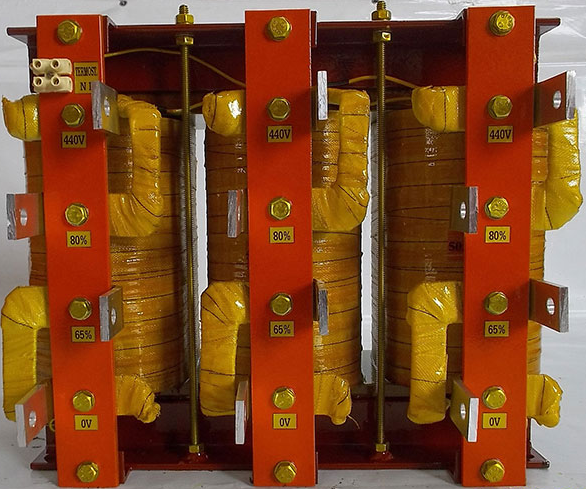
\includegraphics[width=0.7\linewidth]{figuras/autotrafo}
		\caption{Autotransformador trifásico.}
		\label{fig:autotrafo}
	\end{figure}	
\end{frame}

\begin{frame}
\frametitle{Autotransformador}
\framesubtitle{Análise}
	\begin{overprint}
		\only<1>
		{
			\begin{block}{Objetivos}
				\begin{itemize}
					\item Escrever a equação diferencial relacionando a corrente de saída $i_2$ com a tensão de entrada $v_1$.
					\item Calcular as relações de tensão e corrente em estado permanente.
					\item Observação: as bobinas $L_1$ e $L_2$ possuem $N_1$ e $N_2$ espiras, respectivamente.
				\end{itemize}
			\end{block}
			\begin{center}
				\begin{circuitikz}
					% Lower coil
					\draw (0,1.15) to[L] (0,0);
					% Upper coil
					\draw (0,2.30) to[L] (0,1.15);									
					% L1
					\draw node[] at (0.5, 1.725) {$L_1$};
					% L2
					\draw node[] at (0.5, 0.575) {$L_2$};
					% Dot
					\draw node[circ] at (0.35, 2.3) {};
					\draw node[circ] at (0.35, 1) {};
					% Arrow
					\draw [latex-latex] (-0.1,2.3) to [out=240,in=120] (-0.1,1);
					\draw node[] at (-0.6, 1.65) {$M$};
					% Left side
					\draw [thick] (0,2.30) --++ (0,0.5) --++ (-2,0);
					\draw [thick] (0,0) --++ (0,-0.5) --++ (-2,0);	
					\draw (-2,2.8) to[open, v_=$v_1$, *-*] (-2,-0.5);
					% Tap + Right side 
					\draw [thick] (0,1.15) --++ (2.5,0);
					\draw (2.5, 1.15) to[R, l_=$R$, v^=$v_2$] (2.5,-0.5);
					\draw [thick] (0,-0.5) -- (2.5,-0.5);
					% Current i1
					\draw[latex-] (-1,1.15) arc[radius=0.3cm,start angle=0,delta angle=270];
					\draw  (-1, 0.95) node{$i_1$};
					% Current i2
					\draw[latex-] (1.6, 0.4) arc[radius=0.3cm,start angle=0,delta angle=270];
					\draw  (1.6, 0.2) node{$i_2$};
				\end{circuitikz}
			\end{center}
		}
		\only<2>
		{			
			\vspace{-0.1cm}
			\begin{center}
				\begin{circuitikz}[scale=0.8, every node/.style={scale=0.8}]
					% Lower coil
					\draw (0,1.15) to[L] (0,0);
					% Upper coil
					\draw (0,2.30) to[L] (0,1.15);									
					% L1
					\draw node[] at (0.5, 1.725) {$L_1$};
					% L2
					\draw node[] at (0.5, 0.575) {$L_2$};
					% Dot
					\draw node[circ] at (0.35, 2.3) {};
					\draw node[circ] at (0.35, 1) {};
					% Arrow
					\draw [latex-latex] (-0.1,2.3) to [out=240,in=120] (-0.1,1);
					\draw node[] at (-0.6, 1.65) {$M$};
					% Left side
					\draw [thick] (0,2.30) --++ (0,0.5) --++ (-2,0);
					\draw [thick] (0,0) --++ (0,-0.5) --++ (-2,0);	
					\draw (-2,2.8) to[open, v_=$v_1$, *-*] (-2,-0.5);
					% Tap + Right side 
					\draw [thick] (0,1.15) --++ (2.5,0);
					\draw (2.5, 1.15) to[R, l_=$R$, v^=$v_2$] (2.5,-0.5);
					\draw [thick] (0,-0.5) -- (2.5,-0.5);
					% Current i1
					\draw[latex-] (-1,1.15) arc[radius=0.3cm,start angle=0,delta angle=270];
					\draw  (-1, 0.95) node{$i_1$};
					% Current i2
					\draw[latex-] (1.6, 0.4) arc[radius=0.3cm,start angle=0,delta angle=270];
					\draw  (1.6, 0.2) node{$i_2$};
				\end{circuitikz}
			\end{center}
			\vspace{-0.2cm}
			\begin{block}{Equação diferencial}
				\begin{equation}\label{key} \tag{8}
				\left\{ \begin{array}{l}
				{L_1}\frac{{d{i_1}}}{{dt}} + M\left( {\frac{{d{i_1}}}{{dt}} - \frac{{d{i_2}}}{{dt}}} \right) + {L_2}\left( {\frac{{d{i_1}}}{{dt}} - \frac{{d{i_2}}}{{dt}}} \right) + M\frac{{d{i_1}}}{{dt}} = {v_1}\\[5pt]
				R{i_2} + {L_2}\left( {\frac{{d{i_2}}}{{dt}} - \frac{{d{i_1}}}{{dt}}} \right) - M\frac{{d{i_1}}}{{dt}} = 0
				\end{array} \right.
				\end{equation}
				Rearranjando,
				\vspace{-0.4cm}
				\begin{equation}\label{key} \tag{9}
				\left\{ \begin{array}{l}
				\left( {{L_1} + {L_2} + 2M} \right)\frac{{d{i_1}}}{{dt}} - \left( {{L_2} + M} \right)\frac{{d{i_2}}}{{dt}} = {v_1}\\[5pt]
				- \left( {{L_2} + M} \right)\frac{{d{i_1}}}{{dt}} + {L_2}\frac{{d{i_2}}}{{dt}} + R{i_2} = 0
				\end{array} \right.
				\end{equation}
			\end{block}
		}
		\only<3>
		{			
			\vspace{-0.1cm}
			\begin{center}
				\begin{circuitikz}[scale=0.8, every node/.style={scale=0.8}]
					% Lower coil
					\draw (0,1.15) to[L] (0,0);
					% Upper coil
					\draw (0,2.30) to[L] (0,1.15);									
					% L1
					\draw node[] at (0.5, 1.725) {$L_1$};
					% L2
					\draw node[] at (0.5, 0.575) {$L_2$};
					% Dot
					\draw node[circ] at (0.35, 2.3) {};
					\draw node[circ] at (0.35, 1) {};
					% Arrow
					\draw [latex-latex] (-0.1,2.3) to [out=240,in=120] (-0.1,1);
					\draw node[] at (-0.6, 1.65) {$M$};
					% Left side
					\draw [thick] (0,2.30) --++ (0,0.5) --++ (-2,0);
					\draw [thick] (0,0) --++ (0,-0.5) --++ (-2,0);	
					\draw (-2,2.8) to[open, v_=$v_1$, *-*] (-2,-0.5);
					% Tap + Right side 
					\draw [thick] (0,1.15) --++ (2.5,0);
					\draw (2.5, 1.15) to[R, l_=$R$, v^=$v_2$] (2.5,-0.5);
					\draw [thick] (0,-0.5) -- (2.5,-0.5);
					% Current i1
					\draw[latex-] (-1,1.15) arc[radius=0.3cm,start angle=0,delta angle=270];
					\draw  (-1, 0.95) node{$i_1$};
					% Current i2
					\draw[latex-] (1.6, 0.4) arc[radius=0.3cm,start angle=0,delta angle=270];
					\draw  (1.6, 0.2) node{$i_2$};
				\end{circuitikz}
			\end{center}
			\vspace{-0.2cm}
			\begin{block}{Equação diferencial}
				\begin{equation} \label{key} \tag{9}
				\left\{ \begin{array}{l}
				\left( {{L_1} + {L_2} + 2M} \right)\frac{{d{i_1}}}{{dt}} - \left( {{L_2} + M} \right)\frac{{d{i_2}}}{{dt}} = {v_1}\\[5pt]
				- \left( {{L_2} + M} \right)\frac{{d{i_1}}}{{dt}} + {L_2}\frac{{d{i_2}}}{{dt}} + R{i_2} = 0
				\end{array} \right.
				\end{equation}
				Isolando $\frac{di_1}{dt}$ na segunda equação em (9):
				\vspace{-0.3cm}
				\begin{equation}\label{key} \tag{10}
				\left\{ \begin{array}{l}
				\left( {{L_1} + {L_2} + 2M} \right)\frac{{d{i_1}}}{{dt}} - \left( {{L_2} + M} \right)\frac{{d{i_2}}}{{dt}} = {v_1}\\[5pt]
				\frac{{d{i_1}}}{{dt}} = \frac{{{L_2}\frac{{d{i_2}}}{{dt}} + R{i_2}}}{{\left( {{L_2} + M} \right)}}
				\end{array} \right.
				\end{equation}
			\end{block}
		}
		\only<4>
		{			
			\vspace{-0.1cm}
			\begin{center}
				\begin{circuitikz}[scale=0.8, every node/.style={scale=0.8}]
					% Lower coil
					\draw (0,1.15) to[L] (0,0);
					% Upper coil
					\draw (0,2.30) to[L] (0,1.15);									
					% L1
					\draw node[] at (0.5, 1.725) {$L_1$};
					% L2
					\draw node[] at (0.5, 0.575) {$L_2$};
					% Dot
					\draw node[circ] at (0.35, 2.3) {};
					\draw node[circ] at (0.35, 1) {};
					% Arrow
					\draw [latex-latex] (-0.1,2.3) to [out=240,in=120] (-0.1,1);
					\draw node[] at (-0.6, 1.65) {$M$};
					% Left side
					\draw [thick] (0,2.30) --++ (0,0.5) --++ (-2,0);
					\draw [thick] (0,0) --++ (0,-0.5) --++ (-2,0);	
					\draw (-2,2.8) to[open, v_=$v_1$, *-*] (-2,-0.5);
					% Tap + Right side 
					\draw [thick] (0,1.15) --++ (2.5,0);
					\draw (2.5, 1.15) to[R, l_=$R$, v^=$v_2$] (2.5,-0.5);
					\draw [thick] (0,-0.5) -- (2.5,-0.5);
					% Current i1
					\draw[latex-] (-1,1.15) arc[radius=0.3cm,start angle=0,delta angle=270];
					\draw  (-1, 0.95) node{$i_1$};
					% Current i2
					\draw[latex-] (1.6, 0.4) arc[radius=0.3cm,start angle=0,delta angle=270];
					\draw  (1.6, 0.2) node{$i_2$};
				\end{circuitikz}
			\end{center}
			\vspace{-0.2cm}
			\begin{block}{Equação diferencial}
				\begin{equation}\label{key} \tag{10}
				\left\{ \begin{array}{l}
				\left( {{L_1} + {L_2} + 2M} \right)\frac{{d{i_1}}}{{dt}} - \left( {{L_2} + M} \right)\frac{{d{i_2}}}{{dt}} = {v_1}\\[5pt]
				\frac{{d{i_1}}}{{dt}} = \frac{{{L_2}\frac{{d{i_2}}}{{dt}} + R{i_2}}}{{\left( {{L_2} + M} \right)}}
				\end{array} \right.
				\end{equation}
				Substituindo a segunda equação de (10) na primeira:
				\vspace{-0.3cm}
				\begin{equation}\label{key} \tag{11}
				\left( {\frac{{{L_1} + {L_2} + 2M}}{{{L_2} + M}}} \right)\left( {{L_2}\frac{{d{i_2}}}{{dt}} + R{i_2}} \right) - \left( {{L_2} + M} \right)\frac{{d{i_2}}}{{dt}} = {v_1}
				\end{equation}
			\end{block}
		}
		\only<5>
		{			
			\vspace{-0.1cm}
			\begin{center}
				\begin{circuitikz}[scale=0.8, every node/.style={scale=0.8}]
					% Lower coil
					\draw (0,1.15) to[L] (0,0);
					% Upper coil
					\draw (0,2.30) to[L] (0,1.15);									
					% L1
					\draw node[] at (0.5, 1.725) {$L_1$};
					% L2
					\draw node[] at (0.5, 0.575) {$L_2$};
					% Dot
					\draw node[circ] at (0.35, 2.3) {};
					\draw node[circ] at (0.35, 1) {};
					% Arrow
					\draw [latex-latex] (-0.1,2.3) to [out=240,in=120] (-0.1,1);
					\draw node[] at (-0.6, 1.65) {$M$};
					% Left side
					\draw [thick] (0,2.30) --++ (0,0.5) --++ (-2,0);
					\draw [thick] (0,0) --++ (0,-0.5) --++ (-2,0);	
					\draw (-2,2.8) to[open, v_=$v_1$, *-*] (-2,-0.5);
					% Tap + Right side 
					\draw [thick] (0,1.15) --++ (2.5,0);
					\draw (2.5, 1.15) to[R, l_=$R$, v^=$v_2$] (2.5,-0.5);
					\draw [thick] (0,-0.5) -- (2.5,-0.5);
					% Current i1
					\draw[latex-] (-1,1.15) arc[radius=0.3cm,start angle=0,delta angle=270];
					\draw  (-1, 0.95) node{$i_1$};
					% Current i2
					\draw[latex-] (1.6, 0.4) arc[radius=0.3cm,start angle=0,delta angle=270];
					\draw  (1.6, 0.2) node{$i_2$};
				\end{circuitikz}
			\end{center}
			\vspace{-0.2cm}
			\begin{block}{Equação diferencial}
				\begin{equation}\label{key} \tag{11}
				\left( {\frac{{{L_1} + {L_2} + 2M}}{{{L_2} + M}}} \right)\left( {{L_2}\frac{{d{i_2}}}{{dt}} + R{i_2}} \right) - \left( {{L_2} + M} \right)\frac{{d{i_2}}}{{dt}} = {v_1}
				\end{equation}
				Rearranjando,
				\vspace{-0.3cm}
				\begin{equation}\label{key} \tag{12}
				\left( {{L_1}{L_2} - {M^2}} \right)\frac{{d{i_2}}}{{dt}} + R\left( {{L_1} + {L_2} + 2M} \right){i_2} = \left( {{L_2} + M} \right){v_1}
				\end{equation}
			\end{block}
		}
		\only<6>
		{			
			\vspace{-0.1cm}
			\begin{center}
				\begin{circuitikz}[scale=0.8, every node/.style={scale=0.8}]
					% Lower coil
					\draw (0,1.15) to[L] (0,0);
					% Upper coil
					\draw (0,2.30) to[L] (0,1.15);									
					% L1
					\draw node[] at (0.5, 1.725) {$L_1$};
					% L2
					\draw node[] at (0.5, 0.575) {$L_2$};
					% Dot
					\draw node[circ] at (0.35, 2.3) {};
					\draw node[circ] at (0.35, 1) {};
					% Arrow
					\draw [latex-latex] (-0.1,2.3) to [out=240,in=120] (-0.1,1);
					\draw node[] at (-0.6, 1.65) {$M$};
					% Left side
					\draw [thick] (0,2.30) --++ (0,0.5) --++ (-2,0);
					\draw [thick] (0,0) --++ (0,-0.5) --++ (-2,0);	
					\draw (-2,2.8) to[open, v_=$v_1$, *-*] (-2,-0.5);
					% Tap + Right side 
					\draw [thick] (0,1.15) --++ (2.5,0);
					\draw (2.5, 1.15) to[R, l_=$R$, v^=$v_2$] (2.5,-0.5);
					\draw [thick] (0,-0.5) -- (2.5,-0.5);
					% Current i1
					\draw[latex-] (-1,1.15) arc[radius=0.3cm,start angle=0,delta angle=270];
					\draw  (-1, 0.95) node{$i_1$};
					% Current i2
					\draw[latex-] (1.6, 0.4) arc[radius=0.3cm,start angle=0,delta angle=270];
					\draw  (1.6, 0.2) node{$i_2$};
				\end{circuitikz}
			\end{center}
			\vspace{-0.2cm}
			\begin{block}{Equação diferencial}
				\begin{equation}\label{key} \tag{12}
				\left( {{L_1}{L_2} - {M^2}} \right)\frac{{d{i_2}}}{{dt}} + R\left( {{L_1} + {L_2} + 2M} \right){i_2} = \left( {{L_2} + M} \right){v_1}
				\end{equation}
				Considerando o coeficiente de acoplamento unitário ($k=1$ em $M=k\sqrt {{L_1}{L_2}}$), a primeira parcela é anulada.
				\vspace{-0.3cm}
				\begin{equation}\label{key} \tag{13}
				\textcolor{red}{\left( {{L_1}{L_2} - {M^2}} \right)\frac{{d{i_2}}}{{dt}}} + R\left( {{L_1} + {L_2} + 2M} \right){i_2} = \left( {{L_2} + M} \right){v_1}
				\end{equation}
			\end{block}
		}
		\only<7>
		{			
			\vspace{-0.1cm}
			\begin{center}
				\begin{circuitikz}[scale=0.8, every node/.style={scale=0.8}]
					% Lower coil
					\draw (0,1.15) to[L] (0,0);
					% Upper coil
					\draw (0,2.30) to[L] (0,1.15);									
					% L1
					\draw node[] at (0.5, 1.725) {$L_1$};
					% L2
					\draw node[] at (0.5, 0.575) {$L_2$};
					% Dot
					\draw node[circ] at (0.35, 2.3) {};
					\draw node[circ] at (0.35, 1) {};
					% Arrow
					\draw [latex-latex] (-0.1,2.3) to [out=240,in=120] (-0.1,1);
					\draw node[] at (-0.6, 1.65) {$M$};
					% Left side
					\draw [thick] (0,2.30) --++ (0,0.5) --++ (-2,0);
					\draw [thick] (0,0) --++ (0,-0.5) --++ (-2,0);	
					\draw (-2,2.8) to[open, v_=$v_1$, *-*] (-2,-0.5);
					% Tap + Right side 
					\draw [thick] (0,1.15) --++ (2.5,0);
					\draw (2.5, 1.15) to[R, l_=$R$, v^=$v_2$] (2.5,-0.5);
					\draw [thick] (0,-0.5) -- (2.5,-0.5);
					% Current i1
					\draw[latex-] (-1,1.15) arc[radius=0.3cm,start angle=0,delta angle=270];
					\draw  (-1, 0.95) node{$i_1$};
					% Current i2
					\draw[latex-] (1.6, 0.4) arc[radius=0.3cm,start angle=0,delta angle=270];
					\draw  (1.6, 0.2) node{$i_2$};
				\end{circuitikz}
			\end{center}
			\vspace{-0.2cm}
			\begin{block}{Equação diferencial}
				\begin{equation}\label{key} \tag{12}
				\left( {{L_1}{L_2} - {M^2}} \right)\frac{{d{i_2}}}{{dt}} + R\left( {{L_1} + {L_2} + 2M} \right){i_2} = \left( {{L_2} + M} \right){v_1}
				\end{equation}
				Considerando o coeficiente de acoplamento unitário ($k=1$ em $M=k\sqrt {{L_1}{L_2}}$), a primeira parcela é anulada.
				\vspace{-0.3cm}
				\begin{equation}\label{key} \tag{13}
				R\left( {{L_1} + {L_2} + 2M} \right){i_2} = \left( {{L_2} + M} \right){v_1}
				\end{equation}
			\end{block}
		}
		\only<8>
		{			
			\vspace{-0.1cm}
			\begin{center}
				\begin{circuitikz}[scale=0.8, every node/.style={scale=0.8}]
					% Lower coil
					\draw (0,1.15) to[L] (0,0);
					% Upper coil
					\draw (0,2.30) to[L] (0,1.15);									
					% L1
					\draw node[] at (0.5, 1.725) {$L_1$};
					% L2
					\draw node[] at (0.5, 0.575) {$L_2$};
					% Dot
					\draw node[circ] at (0.35, 2.3) {};
					\draw node[circ] at (0.35, 1) {};
					% Arrow
					\draw [latex-latex] (-0.1,2.3) to [out=240,in=120] (-0.1,1);
					\draw node[] at (-0.6, 1.65) {$M$};
					% Left side
					\draw [thick] (0,2.30) --++ (0,0.5) --++ (-2,0);
					\draw [thick] (0,0) --++ (0,-0.5) --++ (-2,0);	
					\draw (-2,2.8) to[open, v_=$v_1$, *-*] (-2,-0.5);
					% Tap + Right side 
					\draw [thick] (0,1.15) --++ (2.5,0);
					\draw (2.5, 1.15) to[R, l_=$R$, v^=$v_2$] (2.5,-0.5);
					\draw [thick] (0,-0.5) -- (2.5,-0.5);
					% Current i1
					\draw[latex-] (-1,1.15) arc[radius=0.3cm,start angle=0,delta angle=270];
					\draw  (-1, 0.95) node{$i_1$};
					% Current i2
					\draw[latex-] (1.6, 0.4) arc[radius=0.3cm,start angle=0,delta angle=270];
					\draw  (1.6, 0.2) node{$i_2$};
				\end{circuitikz}
			\end{center}
			\vspace{-0.2cm}
			\begin{block}{Equação diferencial}
				\begin{equation}\label{key} \tag{13}
				R\left( {{L_1} + {L_2} + 2M} \right){i_2} = \left( {{L_2} + M} \right){v_1}
				\end{equation}
				Portanto,
				\begin{equation}\label{key} \tag{14}
				{i_2} = \frac{{\left( {{L_2} + M} \right)}}{{R\left( {{L_1} + {L_2} + 2M} \right)}}{v_1}
				\end{equation}
			\end{block}
		}
		\only<9>
		{			
			\vspace{-0.1cm}
			\begin{center}
				\begin{circuitikz}[scale=0.8, every node/.style={scale=0.8}]
					% Lower coil
					\draw (0,1.15) to[L] (0,0);
					% Upper coil
					\draw (0,2.30) to[L] (0,1.15);									
					% L1
					\draw node[] at (0.5, 1.725) {$L_1$};
					% L2
					\draw node[] at (0.5, 0.575) {$L_2$};
					% Dot
					\draw node[circ] at (0.35, 2.3) {};
					\draw node[circ] at (0.35, 1) {};
					% Arrow
					\draw [latex-latex] (-0.1,2.3) to [out=240,in=120] (-0.1,1);
					\draw node[] at (-0.6, 1.65) {$M$};
					% Left side
					\draw [thick] (0,2.30) --++ (0,0.5) --++ (-2,0);
					\draw [thick] (0,0) --++ (0,-0.5) --++ (-2,0);	
					\draw (-2,2.8) to[open, v_=$V_1$, *-*] (-2,-0.5);
					% Tap + Right side 
					\draw [thick] (0,1.15) --++ (2.5,0);
					\draw (2.5, 1.15) to[R, l_=$R$, v^=$V_2$] (2.5,-0.5);
					\draw [thick] (0,-0.5) -- (2.5,-0.5);
					% Current i1
					\draw[latex-] (-1,1.15) arc[radius=0.3cm,start angle=0,delta angle=270];
					\draw  (-1, 0.95) node{$I_1$};
					% Current i2
					\draw[latex-] (1.6, 0.4) arc[radius=0.3cm,start angle=0,delta angle=270];
					\draw  (1.6, 0.2) node{$I_2$};
				\end{circuitikz}
			\end{center}
			\vspace{-0.2cm}
			\begin{block}{Em estado permanente senoidal}
				\begin{equation}\label{key} \tag{12}
				\left( {{L_1}{L_2} - {M^2}} \right)\frac{{d{i_2}}}{{dt}} + R\left( {{L_1} + {L_2} + 2M} \right){i_2} = \left( {{L_2} + M} \right){v_1}
				\end{equation}
				Em estado permanente senoidal,
%				\vspace{-0.3cm}
				\begin{equation}\label{key} \tag{15}
				j\omega \left( {{L_1}{L_2} - {M^2}} \right){I_2} + R\left( {{L_1} + {L_2} + 2M} \right){I_2} = \left( {{L_2} + M} \right){V_1}
				\end{equation}
			\end{block}
		}
		\only<10>
		{			
			\vspace{-0.1cm}
			\begin{center}
				\begin{circuitikz}[scale=0.8, every node/.style={scale=0.8}]
					% Lower coil
					\draw (0,1.15) to[L] (0,0);
					% Upper coil
					\draw (0,2.30) to[L] (0,1.15);									
					% L1
					\draw node[] at (0.5, 1.725) {$L_1$};
					% L2
					\draw node[] at (0.5, 0.575) {$L_2$};
					% Dot
					\draw node[circ] at (0.35, 2.3) {};
					\draw node[circ] at (0.35, 1) {};
					% Arrow
					\draw [latex-latex] (-0.1,2.3) to [out=240,in=120] (-0.1,1);
					\draw node[] at (-0.6, 1.65) {$M$};
					% Left side
					\draw [thick] (0,2.30) --++ (0,0.5) --++ (-2,0);
					\draw [thick] (0,0) --++ (0,-0.5) --++ (-2,0);	
					\draw (-2,2.8) to[open, v_=$V_1$, *-*] (-2,-0.5);
					% Tap + Right side 
					\draw [thick] (0,1.15) --++ (2.5,0);
					\draw (2.5, 1.15) to[R, l_=$R$, v^=$V_2$] (2.5,-0.5);
					\draw [thick] (0,-0.5) -- (2.5,-0.5);
					% Current i1
					\draw[latex-] (-1,1.15) arc[radius=0.3cm,start angle=0,delta angle=270];
					\draw  (-1, 0.95) node{$I_1$};
					% Current i2
					\draw[latex-] (1.6, 0.4) arc[radius=0.3cm,start angle=0,delta angle=270];
					\draw  (1.6, 0.2) node{$I_2$};
				\end{circuitikz}
			\end{center}
			\vspace{-0.2cm}
			\begin{block}{Em estado permanente senoidal}
				\begin{equation}\label{key} \tag{15}
				j\omega \left( {{L_1}{L_2} - {M^2}} \right){I_2} + R\left( {{L_1} + {L_2} + 2M} \right){I_2} = \left( {{L_2} + M} \right){V_1}
				\end{equation}
				Rearranjando,
				%				\vspace{-0.3cm}
				\begin{equation}\label{key} \tag{16}
				\frac{{{I_2}}}{{{V_1}}} = \frac{{{L_2} + M}}{{j\omega \left( {{L_1}{L_2} - {M^2}} \right) + R\left( {{L_1} + {L_2} + 2M} \right)}}
				\end{equation}
			\end{block}
		}
		\only<11>
		{			
			\vspace{-0.1cm}
			\begin{center}
				\begin{circuitikz}[scale=0.8, every node/.style={scale=0.8}]
					% Lower coil
					\draw (0,1.15) to[L] (0,0);
					% Upper coil
					\draw (0,2.30) to[L] (0,1.15);									
					% L1
					\draw node[] at (0.5, 1.725) {$L_1$};
					% L2
					\draw node[] at (0.5, 0.575) {$L_2$};
					% Dot
					\draw node[circ] at (0.35, 2.3) {};
					\draw node[circ] at (0.35, 1) {};
					% Arrow
					\draw [latex-latex] (-0.1,2.3) to [out=240,in=120] (-0.1,1);
					\draw node[] at (-0.6, 1.65) {$M$};
					% Left side
					\draw [thick] (0,2.30) --++ (0,0.5) --++ (-2,0);
					\draw [thick] (0,0) --++ (0,-0.5) --++ (-2,0);	
					\draw (-2,2.8) to[open, v_=$V_1$, *-*] (-2,-0.5);
					% Tap + Right side 
					\draw [thick] (0,1.15) --++ (2.5,0);
					\draw (2.5, 1.15) to[R, l_=$R$, v^=$V_2$] (2.5,-0.5);
					\draw [thick] (0,-0.5) -- (2.5,-0.5);
					% Current i1
					\draw[latex-] (-1,1.15) arc[radius=0.3cm,start angle=0,delta angle=270];
					\draw  (-1, 0.95) node{$I_1$};
					% Current i2
					\draw[latex-] (1.6, 0.4) arc[radius=0.3cm,start angle=0,delta angle=270];
					\draw  (1.6, 0.2) node{$I_2$};
				\end{circuitikz}
			\end{center}
			\vspace{-0.2cm}
			\begin{block}{Em estado permanente senoidal}
				\begin{equation}\label{key} \tag{9}
				\left\{ \begin{array}{l}
				\left( {{L_1} + {L_2} + 2M} \right)\frac{{d{i_1}}}{{dt}} - \left( {{L_2} + M} \right)\frac{{d{i_2}}}{{dt}} = {v_1}\\[5pt]
				- \left( {{L_2} + M} \right)\frac{{d{i_1}}}{{dt}} + {L_2}\frac{{d{i_2}}}{{dt}} + R{i_2} = 0
				\end{array} \right.
				\end{equation}
				Da segunda equação de (9):
				%				\vspace{-0.3cm}
				\begin{equation}\label{key} \tag{17}
				- j\omega \left( {{L_2} + M} \right){I_1} + j\omega {L_2}{I_2} + R{I_2} = 0 \Rightarrow \frac{{{I_2}}}{{{I_1}}} = \frac{{j\omega \left( {{L_2} + M} \right)}}{{j\omega {L_2} + R}}
				\end{equation}
			\end{block}
		}
		\only<12>
		{			
			\vspace{-0.1cm}
			\begin{center}
				\begin{circuitikz}[scale=0.8, every node/.style={scale=0.8}]
					% Lower coil
					\draw (0,1.15) to[L] (0,0);
					% Upper coil
					\draw (0,2.30) to[L] (0,1.15);									
					% L1
					\draw node[] at (0.5, 1.725) {$L_1$};
					% L2
					\draw node[] at (0.5, 0.575) {$L_2$};
					% Dot
					\draw node[circ] at (0.35, 2.3) {};
					\draw node[circ] at (0.35, 1) {};
					% Arrow
					\draw [latex-latex] (-0.1,2.3) to [out=240,in=120] (-0.1,1);
					\draw node[] at (-0.6, 1.65) {$M$};
					% Left side
					\draw [thick] (0,2.30) --++ (0,0.5) --++ (-2,0);
					\draw [thick] (0,0) --++ (0,-0.5) --++ (-2,0);	
					\draw (-2,2.8) to[open, v_=$V_1$, *-*] (-2,-0.5);
					% Tap + Right side 
					\draw [thick] (0,1.15) --++ (2.5,0);
					\draw (2.5, 1.15) to[R, l_=$R$, v^=$V_2$] (2.5,-0.5);
					\draw [thick] (0,-0.5) -- (2.5,-0.5);
					% Current i1
					\draw[latex-] (-1,1.15) arc[radius=0.3cm,start angle=0,delta angle=270];
					\draw  (-1, 0.95) node{$I_1$};
					% Current i2
					\draw[latex-] (1.6, 0.4) arc[radius=0.3cm,start angle=0,delta angle=270];
					\draw  (1.6, 0.2) node{$I_2$};
				\end{circuitikz}
			\end{center}
			\vspace{-0.2cm}
			\begin{block}{Em estado permanente senoidal}
				\begin{equation}\label{key} \tag{17}
				- j\omega \left( {{L_2} + M} \right){I_1} + j\omega {L_2}{I_2} + R{I_2} = 0 \Rightarrow \frac{{{I_2}}}{{{I_1}}} = \frac{{j\omega \left( {{L_2} + M} \right)}}{{j\omega {L_2} + R}}
				\end{equation}
				Geralmente, $j\omega L_2 \gg R$. Para um autotransformador ideal ($k = 1$):
				%				\vspace{-0.3cm}
				\begin{equation}\label{key} \tag{18}
				\frac{{{I_2}}}{{{I_1}}} = \frac{{j\omega \left( {{L_2} + M} \right)}}{{j\omega {L_2}}} = 1 + \frac{M}{{{L_2}}} = 1 + \frac{{k\sqrt {{L_1}{L_2}} }}{{{L_2}}} = 1 + \sqrt {\frac{{{L_1}}}{{{L_2}}}}  = 1 + \frac{{{N_1}}}{{{N_2}}}
				\end{equation}
			\end{block}
		}
		\only<13>
		{			
			\vspace{-0.1cm}
			\begin{center}
				\begin{circuitikz}[scale=0.8, every node/.style={scale=0.8}]
					% Lower coil
					\draw (0,1.15) to[L] (0,0);
					% Upper coil
					\draw (0,2.30) to[L] (0,1.15);									
					% L1
					\draw node[] at (0.5, 1.725) {$L_1$};
					% L2
					\draw node[] at (0.5, 0.575) {$L_2$};
					% Dot
					\draw node[circ] at (0.35, 2.3) {};
					\draw node[circ] at (0.35, 1) {};
					% Arrow
					\draw [latex-latex] (-0.1,2.3) to [out=240,in=120] (-0.1,1);
					\draw node[] at (-0.6, 1.65) {$M$};
					% Left side
					\draw [thick] (0,2.30) --++ (0,0.5) --++ (-2,0);
					\draw [thick] (0,0) --++ (0,-0.5) --++ (-2,0);	
					\draw (-2,2.8) to[open, v_=$V_1$, *-*] (-2,-0.5);
					% Tap + Right side 
					\draw [thick] (0,1.15) --++ (2.5,0);
					\draw (2.5, 1.15) to[R, l_=$R$, v^=$V_2$] (2.5,-0.5);
					\draw [thick] (0,-0.5) -- (2.5,-0.5);
					% Current i1
					\draw[latex-] (-1,1.15) arc[radius=0.3cm,start angle=0,delta angle=270];
					\draw  (-1, 0.95) node{$I_1$};
					% Current i2
					\draw[latex-] (1.6, 0.4) arc[radius=0.3cm,start angle=0,delta angle=270];
					\draw  (1.6, 0.2) node{$I_2$};
				\end{circuitikz}
			\end{center}
			\vspace{-0.2cm}
			\begin{block}{Em estado permanente senoidal}
				\begin{equation}\label{key} \tag{17}
				- j\omega \left( {{L_2} + M} \right){I_1} + j\omega {L_2}{I_2} + R{I_2} = 0 \Rightarrow \frac{{{I_2}}}{{{I_1}}} = \frac{{j\omega \left( {{L_2} + M} \right)}}{{j\omega {L_2} + R}}
				\end{equation}
				Geralmente, $j\omega L_2 \gg R$. Para um autotransformador ideal ($k = 1$):
				%				\vspace{-0.3cm}
				\begin{equation}\label{key} \tag{18}
				\frac{{{I_2}}}{{{I_1}}} = 1 + \frac{{{N_1}}}{{{N_2}}} = \frac{{{N_1} + {N_2}}}{{{N_2}}}
				\end{equation}
			\end{block}
		}
		\only<14>
		{			
			\vspace{-0.1cm}
			\begin{center}
				\begin{circuitikz}[scale=0.8, every node/.style={scale=0.8}]
					% Lower coil
					\draw (0,1.15) to[L] (0,0);
					% Upper coil
					\draw (0,2.30) to[L] (0,1.15);									
					% L1
					\draw node[] at (0.5, 1.725) {$L_1$};
					% L2
					\draw node[] at (0.5, 0.575) {$L_2$};
					% Dot
					\draw node[circ] at (0.35, 2.3) {};
					\draw node[circ] at (0.35, 1) {};
					% Arrow
					\draw [latex-latex] (-0.1,2.3) to [out=240,in=120] (-0.1,1);
					\draw node[] at (-0.6, 1.65) {$M$};
					% Left side
					\draw [thick] (0,2.30) --++ (0,0.5) --++ (-2,0);
					\draw [thick] (0,0) --++ (0,-0.5) --++ (-2,0);	
					\draw (-2,2.8) to[open, v_=$V_1$, *-*] (-2,-0.5);
					% Tap + Right side 
					\draw [thick] (0,1.15) --++ (2.5,0);
					\draw (2.5, 1.15) to[R, l_=$R$, v^=$V_2$] (2.5,-0.5);
					\draw [thick] (0,-0.5) -- (2.5,-0.5);
					% Current i1
					\draw[latex-] (-1,1.15) arc[radius=0.3cm,start angle=0,delta angle=270];
					\draw  (-1, 0.95) node{$I_1$};
					% Current i2
					\draw[latex-] (1.6, 0.4) arc[radius=0.3cm,start angle=0,delta angle=270];
					\draw  (1.6, 0.2) node{$I_2$};
				\end{circuitikz}
			\end{center}
			\vspace{-0.2cm}
			\begin{block}{Em estado permanente senoidal}
				\begin{equation}\label{key} \tag{16}
				\frac{{{I_2}}}{{{V_1}}} = \frac{{{L_2} + M}}{{j\omega \left( {{L_1}{L_2} - {M^2}} \right) + R\left( {{L_1} + {L_2} + 2M} \right)}}
				\end{equation}
				A relação entre as tensões é dada por:
				%				\vspace{-0.3cm}
				\begin{equation}\label{key} \tag{19}
				\frac{{{V_2}}}{{{V_1}}} = \frac{{R{I_2}}}{{{V_1}}} = \frac{{R\left( {{L_2} + M} \right)}}{{j\omega \left( {{L_1}{L_2} - {M^2}} \right) + R\left( {{L_1} + {L_2} + 2M} \right)}}
				\end{equation}
			\end{block}
		}
		\only<15>
		{			
			\vspace{-0.1cm}
			\begin{center}
				\begin{circuitikz}[scale=0.8, every node/.style={scale=0.8}]
					% Lower coil
					\draw (0,1.15) to[L] (0,0);
					% Upper coil
					\draw (0,2.30) to[L] (0,1.15);									
					% L1
					\draw node[] at (0.5, 1.725) {$L_1$};
					% L2
					\draw node[] at (0.5, 0.575) {$L_2$};
					% Dot
					\draw node[circ] at (0.35, 2.3) {};
					\draw node[circ] at (0.35, 1) {};
					% Arrow
					\draw [latex-latex] (-0.1,2.3) to [out=240,in=120] (-0.1,1);
					\draw node[] at (-0.6, 1.65) {$M$};
					% Left side
					\draw [thick] (0,2.30) --++ (0,0.5) --++ (-2,0);
					\draw [thick] (0,0) --++ (0,-0.5) --++ (-2,0);	
					\draw (-2,2.8) to[open, v_=$V_1$, *-*] (-2,-0.5);
					% Tap + Right side 
					\draw [thick] (0,1.15) --++ (2.5,0);
					\draw (2.5, 1.15) to[R, l_=$R$, v^=$V_2$] (2.5,-0.5);
					\draw [thick] (0,-0.5) -- (2.5,-0.5);
					% Current i1
					\draw[latex-] (-1,1.15) arc[radius=0.3cm,start angle=0,delta angle=270];
					\draw  (-1, 0.95) node{$I_1$};
					% Current i2
					\draw[latex-] (1.6, 0.4) arc[radius=0.3cm,start angle=0,delta angle=270];
					\draw  (1.6, 0.2) node{$I_2$};
				\end{circuitikz}
			\end{center}
			\vspace{-0.2cm}
			\begin{block}{Em estado permanente senoidal}
				\begin{equation}\label{key} \tag{19}
				\frac{{{V_2}}}{{{V_1}}} = \frac{{R{I_2}}}{{{V_1}}} = \frac{{R\left( {{L_2} + M} \right)}}{{j\omega \left( {{L_1}{L_2} - {M^2}} \right) + R\left( {{L_1} + {L_2} + 2M} \right)}}
				\end{equation}
				Para um autotransformador ideal:
				%				\vspace{-0.3cm}
				\begin{equation}\label{key} \tag{20}
				\frac{{{V_2}}}{{{V_1}}} = \frac{{R\left( {{L_2} + M} \right)}}{{R\left( {{L_1} + {L_2} + 2M} \right)}} = \frac{{{L_2} + M}}{{{L_1} + {L_2} + 2M}} = \frac{{{L_2}\left( {1 + \frac{M}{{{L_2}}}} \right)}}{{{L_2}\left( {\frac{{{L_1}}}{{{L_2}}} + 1 + \frac{{2M}}{2}} \right)}}
				\end{equation}
			\end{block}
		}
		\only<16>
		{			
			\vspace{-0.1cm}
			\begin{center}
				\begin{circuitikz}[scale=0.8, every node/.style={scale=0.8}]
					% Lower coil
					\draw (0,1.15) to[L] (0,0);
					% Upper coil
					\draw (0,2.30) to[L] (0,1.15);									
					% L1
					\draw node[] at (0.5, 1.725) {$L_1$};
					% L2
					\draw node[] at (0.5, 0.575) {$L_2$};
					% Dot
					\draw node[circ] at (0.35, 2.3) {};
					\draw node[circ] at (0.35, 1) {};
					% Arrow
					\draw [latex-latex] (-0.1,2.3) to [out=240,in=120] (-0.1,1);
					\draw node[] at (-0.6, 1.65) {$M$};
					% Left side
					\draw [thick] (0,2.30) --++ (0,0.5) --++ (-2,0);
					\draw [thick] (0,0) --++ (0,-0.5) --++ (-2,0);	
					\draw (-2,2.8) to[open, v_=$V_1$, *-*] (-2,-0.5);
					% Tap + Right side 
					\draw [thick] (0,1.15) --++ (2.5,0);
					\draw (2.5, 1.15) to[R, l_=$R$, v^=$V_2$] (2.5,-0.5);
					\draw [thick] (0,-0.5) -- (2.5,-0.5);
					% Current i1
					\draw[latex-] (-1,1.15) arc[radius=0.3cm,start angle=0,delta angle=270];
					\draw  (-1, 0.95) node{$I_1$};
					% Current i2
					\draw[latex-] (1.6, 0.4) arc[radius=0.3cm,start angle=0,delta angle=270];
					\draw  (1.6, 0.2) node{$I_2$};
				\end{circuitikz}
			\end{center}
			\vspace{-0.2cm}
			\begin{block}{Em estado permanente senoidal}
				\begin{equation}\label{key} \tag{19}
				\frac{{{V_2}}}{{{V_1}}} = \frac{{R{I_2}}}{{{V_1}}} = \frac{{R\left( {{L_2} + M} \right)}}{{j\omega \left( {{L_1}{L_2} - {M^2}} \right) + R\left( {{L_1} + {L_2} + 2M} \right)}}
				\end{equation}
				Para um autotransformador ideal:
				%				\vspace{-0.3cm}
				\begin{equation}\label{key} \tag{20}
				\frac{{{V_2}}}{{{V_1}}} = \frac{{{L_2}\left( {1 + \frac{M}{{{L_2}}}} \right)}}{{{L_2}\left( {\frac{{{L_1}}}{{{L_2}}} + 1 + \frac{{2M}}{{{L_2}}}} \right)}} = \frac{{{L_2}\left( {1 + \frac{{\sqrt {{L_1}{L_2}} }}{{{L_2}}}} \right)}}{{{L_2}\left( {\frac{{{L_1}}}{{{L_2}}} + 1 + \frac{{2\sqrt {{L_1}{L_2}} }}{{{L_2}}}} \right)}}
				\end{equation}
			\end{block}
		}
		\only<17>
		{			
			\vspace{-0.1cm}
			\begin{center}
				\begin{circuitikz}[scale=0.8, every node/.style={scale=0.8}]
					% Lower coil
					\draw (0,1.15) to[L] (0,0);
					% Upper coil
					\draw (0,2.30) to[L] (0,1.15);									
					% L1
					\draw node[] at (0.5, 1.725) {$L_1$};
					% L2
					\draw node[] at (0.5, 0.575) {$L_2$};
					% Dot
					\draw node[circ] at (0.35, 2.3) {};
					\draw node[circ] at (0.35, 1) {};
					% Arrow
					\draw [latex-latex] (-0.1,2.3) to [out=240,in=120] (-0.1,1);
					\draw node[] at (-0.6, 1.65) {$M$};
					% Left side
					\draw [thick] (0,2.30) --++ (0,0.5) --++ (-2,0);
					\draw [thick] (0,0) --++ (0,-0.5) --++ (-2,0);	
					\draw (-2,2.8) to[open, v_=$V_1$, *-*] (-2,-0.5);
					% Tap + Right side 
					\draw [thick] (0,1.15) --++ (2.5,0);
					\draw (2.5, 1.15) to[R, l_=$R$, v^=$V_2$] (2.5,-0.5);
					\draw [thick] (0,-0.5) -- (2.5,-0.5);
					% Current i1
					\draw[latex-] (-1,1.15) arc[radius=0.3cm,start angle=0,delta angle=270];
					\draw  (-1, 0.95) node{$I_1$};
					% Current i2
					\draw[latex-] (1.6, 0.4) arc[radius=0.3cm,start angle=0,delta angle=270];
					\draw  (1.6, 0.2) node{$I_2$};
				\end{circuitikz}
			\end{center}
			\vspace{-0.2cm}
			\begin{block}{Em estado permanente senoidal}
				\begin{equation}\label{key} \tag{19}
				\frac{{{V_2}}}{{{V_1}}} = \frac{{R{I_2}}}{{{V_1}}} = \frac{{R\left( {{L_2} + M} \right)}}{{j\omega \left( {{L_1}{L_2} - {M^2}} \right) + R\left( {{L_1} + {L_2} + 2M} \right)}}
				\end{equation}
				Para um autotransformador ideal:
				%				\vspace{-0.3cm}
				\begin{equation}\label{key} \tag{20}
				\frac{{{V_2}}}{{{V_1}}} = \frac{{{L_2}\left( {1 + \frac{{\sqrt {{L_1}{L_2}} }}{{{L_2}}}} \right)}}{{{L_2}\left( {\frac{{{L_1}}}{{{L_2}}} + 1 + \frac{{2\sqrt {{L_1}{L_2}} }}{{{L_2}}}} \right)}} = \frac{{{L_2}\left( {1 + \sqrt {\frac{{{L_1}}}{{{L_2}}}} } \right)}}{{{L_2}\left( {\frac{{{L_1}}}{{{L_2}}} + 1 + 2\sqrt {\frac{{{L_1}}}{{{L_2}}}} } \right)}}
				\end{equation}
			\end{block}
		}
		\only<18>
		{			
			\vspace{-0.1cm}
			\begin{center}
				\begin{circuitikz}[scale=0.8, every node/.style={scale=0.8}]
					% Lower coil
					\draw (0,1.15) to[L] (0,0);
					% Upper coil
					\draw (0,2.30) to[L] (0,1.15);									
					% L1
					\draw node[] at (0.5, 1.725) {$L_1$};
					% L2
					\draw node[] at (0.5, 0.575) {$L_2$};
					% Dot
					\draw node[circ] at (0.35, 2.3) {};
					\draw node[circ] at (0.35, 1) {};
					% Arrow
					\draw [latex-latex] (-0.1,2.3) to [out=240,in=120] (-0.1,1);
					\draw node[] at (-0.6, 1.65) {$M$};
					% Left side
					\draw [thick] (0,2.30) --++ (0,0.5) --++ (-2,0);
					\draw [thick] (0,0) --++ (0,-0.5) --++ (-2,0);	
					\draw (-2,2.8) to[open, v_=$V_1$, *-*] (-2,-0.5);
					% Tap + Right side 
					\draw [thick] (0,1.15) --++ (2.5,0);
					\draw (2.5, 1.15) to[R, l_=$R$, v^=$V_2$] (2.5,-0.5);
					\draw [thick] (0,-0.5) -- (2.5,-0.5);
					% Current i1
					\draw[latex-] (-1,1.15) arc[radius=0.3cm,start angle=0,delta angle=270];
					\draw  (-1, 0.95) node{$I_1$};
					% Current i2
					\draw[latex-] (1.6, 0.4) arc[radius=0.3cm,start angle=0,delta angle=270];
					\draw  (1.6, 0.2) node{$I_2$};
				\end{circuitikz}
			\end{center}
			\vspace{-0.2cm}
			\begin{block}{Em estado permanente senoidal}
				\begin{equation}\label{key} \tag{19}
				\frac{{{V_2}}}{{{V_1}}} = \frac{{R{I_2}}}{{{V_1}}} = \frac{{R\left( {{L_2} + M} \right)}}{{j\omega \left( {{L_1}{L_2} - {M^2}} \right) + R\left( {{L_1} + {L_2} + 2M} \right)}}
				\end{equation}
				Para um autotransformador ideal:
				%				\vspace{-0.3cm}
				\begin{equation}\label{key} \tag{20}
				\frac{{{V_2}}}{{{V_1}}} = \frac{{{L_2}\left( {1 + \frac{{\sqrt {{L_1}{L_2}} }}{{{L_2}}}} \right)}}{{{L_2}\left( {\frac{{{L_1}}}{{{L_2}}} + 1 + \frac{{2\sqrt {{L_1}{L_2}} }}{{{L_2}}}} \right)}} = \frac{{{L_2}\left( {1 + \sqrt {\frac{{{L_1}}}{{{L_2}}}} } \right)}}{{{L_2}{{\left( {1 + \sqrt {\frac{{{L_1}}}{{{L_2}}}} } \right)}^2}}} = \frac{1}{{1 + \sqrt {\frac{{{L_1}}}{{{L_2}}}} }}
				\end{equation}
			\end{block}
		}
		\only<19>
		{			
			\vspace{-0.1cm}
			\begin{center}
				\begin{circuitikz}[scale=0.8, every node/.style={scale=0.8}]
					% Lower coil
					\draw (0,1.15) to[L] (0,0);
					% Upper coil
					\draw (0,2.30) to[L] (0,1.15);									
					% L1
					\draw node[] at (0.5, 1.725) {$L_1$};
					% L2
					\draw node[] at (0.5, 0.575) {$L_2$};
					% Dot
					\draw node[circ] at (0.35, 2.3) {};
					\draw node[circ] at (0.35, 1) {};
					% Arrow
					\draw [latex-latex] (-0.1,2.3) to [out=240,in=120] (-0.1,1);
					\draw node[] at (-0.6, 1.65) {$M$};
					% Left side
					\draw [thick] (0,2.30) --++ (0,0.5) --++ (-2,0);
					\draw [thick] (0,0) --++ (0,-0.5) --++ (-2,0);	
					\draw (-2,2.8) to[open, v_=$V_1$, *-*] (-2,-0.5);
					% Tap + Right side 
					\draw [thick] (0,1.15) --++ (2.5,0);
					\draw (2.5, 1.15) to[R, l_=$R$, v^=$V_2$] (2.5,-0.5);
					\draw [thick] (0,-0.5) -- (2.5,-0.5);
					% Current i1
					\draw[latex-] (-1,1.15) arc[radius=0.3cm,start angle=0,delta angle=270];
					\draw  (-1, 0.95) node{$I_1$};
					% Current i2
					\draw[latex-] (1.6, 0.4) arc[radius=0.3cm,start angle=0,delta angle=270];
					\draw  (1.6, 0.2) node{$I_2$};
				\end{circuitikz}
			\end{center}
			\vspace{-0.2cm}
			\begin{block}{Em estado permanente senoidal}
				\begin{equation}\label{key} \tag{19}
				\frac{{{V_2}}}{{{V_1}}} = \frac{{R{I_2}}}{{{V_1}}} = \frac{{R\left( {{L_2} + M} \right)}}{{j\omega \left( {{L_1}{L_2} - {M^2}} \right) + R\left( {{L_1} + {L_2} + 2M} \right)}}
				\end{equation}
				Para um autotransformador ideal:
				%				\vspace{-0.3cm}
				\begin{equation}\label{key} \tag{20}
				\frac{{{V_2}}}{{{V_1}}} = \frac{{{L_2}\left( {1 + \frac{{\sqrt {{L_1}{L_2}} }}{{{L_2}}}} \right)}}{{{L_2}\left( {\frac{{{L_1}}}{{{L_2}}} + 1 + \frac{{2\sqrt {{L_1}{L_2}} }}{{{L_2}}}} \right)}} = \frac{{{L_2}\left( {1 + \sqrt {\frac{{{L_1}}}{{{L_2}}}} } \right)}}{{{L_2}{{\left( {1 + \sqrt {\frac{{{L_1}}}{{{L_2}}}} } \right)}^2}}} = \frac{1}{{1 + \sqrt {\frac{{{L_1}}}{{{L_2}}}} }}
				\end{equation}
			\end{block}
		}
		\only<20>
		{			
			\vspace{-0.1cm}
			\begin{center}
				\begin{circuitikz}[scale=0.8, every node/.style={scale=0.8}]
					% Lower coil
					\draw (0,1.15) to[L] (0,0);
					% Upper coil
					\draw (0,2.30) to[L] (0,1.15);									
					% L1
					\draw node[] at (0.5, 1.725) {$L_1$};
					% L2
					\draw node[] at (0.5, 0.575) {$L_2$};
					% Dot
					\draw node[circ] at (0.35, 2.3) {};
					\draw node[circ] at (0.35, 1) {};
					% Arrow
					\draw [latex-latex] (-0.1,2.3) to [out=240,in=120] (-0.1,1);
					\draw node[] at (-0.6, 1.65) {$M$};
					% Left side
					\draw [thick] (0,2.30) --++ (0,0.5) --++ (-2,0);
					\draw [thick] (0,0) --++ (0,-0.5) --++ (-2,0);	
					\draw (-2,2.8) to[open, v_=$V_1$, *-*] (-2,-0.5);
					% Tap + Right side 
					\draw [thick] (0,1.15) --++ (2.5,0);
					\draw (2.5, 1.15) to[R, l_=$R$, v^=$V_2$] (2.5,-0.5);
					\draw [thick] (0,-0.5) -- (2.5,-0.5);
					% Current i1
					\draw[latex-] (-1,1.15) arc[radius=0.3cm,start angle=0,delta angle=270];
					\draw  (-1, 0.95) node{$I_1$};
					% Current i2
					\draw[latex-] (1.6, 0.4) arc[radius=0.3cm,start angle=0,delta angle=270];
					\draw  (1.6, 0.2) node{$I_2$};
				\end{circuitikz}
			\end{center}
			\vspace{-0.2cm}
			\begin{block}{Em estado permanente senoidal}
				\begin{equation}\label{key} \tag{19}
				\frac{{{V_2}}}{{{V_1}}} = \frac{{R{I_2}}}{{{V_1}}} = \frac{{R\left( {{L_2} + M} \right)}}{{j\omega \left( {{L_1}{L_2} - {M^2}} \right) + R\left( {{L_1} + {L_2} + 2M} \right)}}
				\end{equation}
				Para um autotransformador ideal:
				%				\vspace{-0.3cm}
				\begin{equation}\label{key} \tag{20}
				\frac{{{V_2}}}{{{V_1}}} = \frac{1}{{1 + \sqrt {\frac{{{L_1}}}{{{L_2}}}} }} = \frac{1}{{1 + \frac{{{N_1}}}{{{N_2}}}}} = \frac{{{N_2}}}{{{N_1} + {N_2}}}
				\end{equation}
			\end{block}
		}
		\only<21>
		{			
			\vspace{-0.1cm}
			\begin{center}
				\begin{circuitikz}[scale=0.8, every node/.style={scale=0.8}]
					% Lower coil
					\draw (0,1.15) to[L] (0,0);
					% Upper coil
					\draw (0,2.30) to[L] (0,1.15);									
					% L1
					\draw node[] at (0.5, 1.725) {$L_1$};
					% L2
					\draw node[] at (0.5, 0.575) {$L_2$};
					% Dot
					\draw node[circ] at (0.35, 2.3) {};
					\draw node[circ] at (0.35, 1) {};
					% Arrow
					\draw [latex-latex] (-0.1,2.3) to [out=240,in=120] (-0.1,1);
					\draw node[] at (-0.6, 1.65) {$M$};
					% Left side
					\draw [thick] (0,2.30) --++ (0,0.5) --++ (-2,0);
					\draw [thick] (0,0) --++ (0,-0.5) --++ (-2,0);	
					\draw (-2,2.8) to[open, v_=$V_1$, *-*] (-2,-0.5);
					% Tap + Right side 
					\draw [thick] (0,1.15) --++ (2.5,0);
					\draw (2.5, 1.15) to[R, l_=$R$, v^=$V_2$] (2.5,-0.5);
					\draw [thick] (0,-0.5) -- (2.5,-0.5);
					% Current i1
					\draw[latex-] (-1,1.15) arc[radius=0.3cm,start angle=0,delta angle=270];
					\draw  (-1, 0.95) node{$I_1$};
					% Current i2
					\draw[latex-] (1.6, 0.4) arc[radius=0.3cm,start angle=0,delta angle=270];
					\draw  (1.6, 0.2) node{$I_2$};
				\end{circuitikz}
			\end{center}
			\vspace{-0.2cm}
			\begin{block}{Em estado permanente senoidal}
				Relembrando:\\
				\begin{minipage}[b]{0.45\linewidth}
					\begin{align}\label{key} \tag{18}
					\begin{split}
					\frac{{{I_2}}}{{{I_1}}} = \frac{{{N_1} + {N_2}}}{{{N_2}}}\\
					{I_1} = \frac{{{N_2}}}{{{N_1} + {N_2}}}{I_2}
					\end{split}
					\end{align}
				\end{minipage}
				\hfill
				\begin{minipage}[b]{0.45\linewidth}
					\begin{align}\label{key} \tag{20}
					\begin{split}
					\frac{{{V_2}}}{{{V_1}}} = \frac{{{N_2}}}{{{N_1} + {N_2}}}\\
					{V_1} = \frac{{{N_1} + {N_2}}}{{{N_2}}}{V_2}
					\end{split}
					\end{align}
				\end{minipage}
			\end{block}
		}
		\only<22>
		{			
			\vspace{-0.1cm}
			\begin{center}
				\begin{circuitikz}[scale=0.8, every node/.style={scale=0.8}]
					% Lower coil
					\draw (0,1.15) to[L] (0,0);
					% Upper coil
					\draw (0,2.30) to[L] (0,1.15);									
					% L1
					\draw node[] at (0.5, 1.725) {$L_1$};
					% L2
					\draw node[] at (0.5, 0.575) {$L_2$};
					% Dot
					\draw node[circ] at (0.35, 2.3) {};
					\draw node[circ] at (0.35, 1) {};
					% Arrow
					\draw [latex-latex] (-0.1,2.3) to [out=240,in=120] (-0.1,1);
					\draw node[] at (-0.6, 1.65) {$M$};
					% Left side
					\draw [thick] (0,2.30) --++ (0,0.5) --++ (-2,0);
					\draw [thick] (0,0) --++ (0,-0.5) --++ (-2,0);	
					\draw (-2,2.8) to[open, v_=$V_1$, *-*] (-2,-0.5);
					% Tap + Right side 
					\draw [thick] (0,1.15) --++ (2.5,0);
					\draw (2.5, 1.15) to[R, l_=$R$, v^=$V_2$] (2.5,-0.5);
					\draw [thick] (0,-0.5) -- (2.5,-0.5);
					% Current i1
					\draw[latex-] (-1,1.15) arc[radius=0.3cm,start angle=0,delta angle=270];
					\draw  (-1, 0.95) node{$I_1$};
					% Current i2
					\draw[latex-] (1.6, 0.4) arc[radius=0.3cm,start angle=0,delta angle=270];
					\draw  (1.6, 0.2) node{$I_2$};
				\end{circuitikz}
			\end{center}
			\vspace{-0.2cm}
			\begin{block}{Em estado permanente senoidal}
				\begin{minipage}[b]{0.45\linewidth}
					\begin{equation}\label{key} \tag{18}					
					{I_1} = \frac{{{N_2}}}{{{N_1} + {N_2}}}{I_2}
					\end{equation}
				\end{minipage}
				\hfill
				\begin{minipage}[b]{0.45\linewidth}
					\begin{equation}\label{key} \tag{20}
					{V_1} = \frac{{{N_1} + {N_2}}}{{{N_2}}}{V_2}
					\end{equation}
				\end{minipage}
				Portanto,
				\begin{equation}\label{key} \tag{21}					
					\frac{{{V_1}}}{{{I_1}}} = \frac{{\frac{{{N_1} + {N_2}}}{{{N_2}}}{V_2}}}{{\frac{{{N_2}}}{{{N_1} + {N_2}}}{I_2}}} = {\left( {\frac{{{N_1} + {N_2}}}{{{N_2}}}} \right)^2}\frac{{{V_2}}}{{{I_2}}} = {\left( {\frac{{{N_1} + {N_2}}}{{{N_2}}}} \right)^2}R
				\end{equation}
			\end{block}
		}
		\only<23>
		{			
			\vspace{-0.1cm}
			\begin{center}
				\begin{circuitikz}[scale=0.8, every node/.style={scale=0.8}]
					% Lower coil
					\draw (0,1.15) to[L] (0,0);
					% Upper coil
					\draw (0,2.30) to[L] (0,1.15);									
					% L1
					\draw node[] at (0.5, 1.725) {$L_1$};
					% L2
					\draw node[] at (0.5, 0.575) {$L_2$};
					% Dot
					\draw node[circ] at (0.35, 2.3) {};
					\draw node[circ] at (0.35, 1) {};
					% Arrow
					\draw [latex-latex] (-0.1,2.3) to [out=240,in=120] (-0.1,1);
					\draw node[] at (-0.6, 1.65) {$M$};
					% Left side
					\draw [thick] (0,2.30) --++ (0,0.5) --++ (-2,0);
					\draw [thick] (0,0) --++ (0,-0.5) --++ (-2,0);	
					\draw (-2,2.8) to[open, v_=$V_1$, *-*] (-2,-0.5);
					% Tap + Right side 
					\draw [thick] (0,1.15) --++ (2.5,0);
					\draw (2.5, 1.15) to[R, l_=$R$, v^=$V_2$] (2.5,-0.5);
					\draw [thick] (0,-0.5) -- (2.5,-0.5);
					% Current i1
					\draw[latex-] (-1,1.15) arc[radius=0.3cm,start angle=0,delta angle=270];
					\draw  (-1, 0.95) node{$I_1$};
					% Current i2
					\draw[latex-] (1.6, 0.4) arc[radius=0.3cm,start angle=0,delta angle=270];
					\draw  (1.6, 0.2) node{$I_2$};
				\end{circuitikz}
			\end{center}
			\vspace{-0.2cm}
			\begin{block}{Em estado permanente senoidal}
				Resumindo, \\
				\begin{minipage}[b]{0.45\linewidth}
					\begin{equation}\label{key} \tag{18}					
					\frac{{{I_2}}}{{{I_1}}} = \frac{{{N_1} + {N_2}}}{{{N_2}}}
					\end{equation}
				\end{minipage}
				\hfill
				\begin{minipage}[b]{0.45\linewidth}
					\begin{equation}\label{key} \tag{20}
					\frac{{{V_2}}}{{{V_1}}} = \frac{{{N_2}}}{{{N_1} + {N_2}}}
					\end{equation}
				\end{minipage}
				\begin{equation}\label{key} \tag{21}					
				\frac{{{V_1}}}{{{I_1}}} = {\left( {\frac{{{N_1} + {N_2}}}{{{N_2}}}} \right)^2}R
				\end{equation}
			\end{block}
		}
	\end{overprint}
\end{frame}
%------------------------------------------------
\section{Exercício}
\begin{frame}
\frametitle{Sumário}
\small
\tableofcontents[currentsection]
\end{frame}
%------------------------------------------------
\begin{frame}
\frametitle{Exercício}
\begin{overprint}
	\only<1>
	{
		\begin{block}{Exercício}
			Calcule $I_1$, $I_2$ e $I_0$, sendo que as bobinas $L_1$ e $L_2$ possuem $N_1=100$ e $N_2=60$.  	
			\begin{center}
				\begin{circuitikz}%[scale=0.8, every node/.style={scale=0.8}]
					% Lower coil
					\draw (0,1.15) to[L] (0,0);
					% Upper coil
					\draw (0,2.30) to[L] (0,1.15);									
					% L1
					\draw node[] at (0.5, 1.725) {$L_1$};
					% L2
					\draw node[] at (0.5, 0.575) {$L_2$};
					% Dot
					\draw node[circ] at (0.35, 2.3) {};
					\draw node[circ] at (0.35, 1) {};
					% Arrow
					%			\draw [latex-latex] (-0.1,2.3) to [out=240,in=120] (-0.1,1);
					%			\draw node[] at (-0.6, 1.65) {$M$};
					% Left side
					\draw [thick] (0,2.30) --++ (0,0.5) --++ (-2,0);
					\draw [thick] (0,0) --++ (0,-2.15) --++ (-2,0);	
					\draw (-2,2.8) to[V, l_=$80\angle {0^o}V$] (-2,-2.15);
					% Tap + Right side 
					\draw [thick] (0,1.15) --++ (2.5,0);
					\draw (2.5, 1.15) to[R, l_=$3\Omega$] (2.5,-0.5);
					\draw (2.5,-0.5) to[L, l_=$j4\Omega$] (2.5,-2.15);
					\draw [thick] (0,-2.15) -- (2.5,-2.15);
					% Current i1
					\draw[latex-] (-0.5,0.3) arc[radius=0.3cm,start angle=0,delta angle=270];
					\draw  (-0.4, 0.1) node{$I_1$};
					% Current i2
					\draw[latex-] (1.6, -0.4) arc[radius=0.3cm,start angle=0,delta angle=270];
					\draw  (1.6, -0.6) node{$I_2$};
					% Voltage v2
					\draw (2.5, 1.5) to[open, v^=$V_2$] (2.5,-2.5);
					% Current i0
					\draw [-latex] (-0.25,-2) -- (-0.25, -1) node[midway, left] {$I_0$};
				\end{circuitikz}
			\end{center}
		\end{block}
	}
	\only<2>
	{
		\begin{block}{Exercício}
			\begin{center}
				\begin{circuitikz}[scale=0.7, every node/.style={scale=0.7}]
					% Lower coil
					\draw (0,1.15) to[L] (0,0);
					% Upper coil
					\draw (0,2.30) to[L] (0,1.15);									
					% L1
					\draw node[] at (0.5, 1.725) {$L_1$};
					% L2
					\draw node[] at (0.5, 0.575) {$L_2$};
					% Dot
					\draw node[circ] at (0.35, 2.3) {};
					\draw node[circ] at (0.35, 1) {};
					% Arrow
					%			\draw [latex-latex] (-0.1,2.3) to [out=240,in=120] (-0.1,1);
					%			\draw node[] at (-0.6, 1.65) {$M$};
					% Left side
					\draw [thick] (0,2.30) --++ (0,0.5) --++ (-2,0);
					\draw [thick] (0,0) --++ (0,-2.15) --++ (-2,0);	
					\draw (-2,2.8) to[V, l_=$80\angle {0^o}V$] (-2,-2.15);
					% Tap + Right side 
					\draw [thick] (0,1.15) --++ (2.5,0);
					\draw (2.5, 1.15) to[R, l_=$3\Omega$] (2.5,-0.5);
					\draw (2.5,-0.5) to[L, l_=$j4\Omega$] (2.5,-2.15);
					\draw [thick] (0,-2.15) -- (2.5,-2.15);
					% Current i1
					\draw[latex-] (-0.5,0.3) arc[radius=0.3cm,start angle=0,delta angle=270];
					\draw  (-0.4, 0.1) node{$I_1$};
					% Current i2
					\draw[latex-] (1.6, -0.4) arc[radius=0.3cm,start angle=0,delta angle=270];
					\draw  (1.6, -0.6) node{$I_2$};
					% Voltage v2
					\draw (2.5, 1.5) to[open, v^=$V_2$] (2.5,-2.5);
					% Current i0
					\draw [-latex] (-0.25,-2) -- (-0.25, -1) node[midway, left] {$I_0$};
				\end{circuitikz}
			\end{center}
			\begin{equation*}\label{key}
			\frac{{{V_2}}}{{{V_1}}} = \frac{{{N_2}}}{{{N_1} + {N_2}}} \Rightarrow {V_2} = \frac{{{N_2}}}{{{N_1} + {N_2}}}{V_1} = \frac{{60}}{{60 + 100}} \cdot 80\angle {0^o} = 30\angle {0^o}~V
			\end{equation*}
		\end{block}
	}
	\only<3>
	{
		\begin{block}{Exercício}
			\begin{center}
				\begin{circuitikz}[scale=0.7, every node/.style={scale=0.7}]
					% Lower coil
					\draw (0,1.15) to[L] (0,0);
					% Upper coil
					\draw (0,2.30) to[L] (0,1.15);									
					% L1
					\draw node[] at (0.5, 1.725) {$L_1$};
					% L2
					\draw node[] at (0.5, 0.575) {$L_2$};
					% Dot
					\draw node[circ] at (0.35, 2.3) {};
					\draw node[circ] at (0.35, 1) {};
					% Arrow
					%			\draw [latex-latex] (-0.1,2.3) to [out=240,in=120] (-0.1,1);
					%			\draw node[] at (-0.6, 1.65) {$M$};
					% Left side
					\draw [thick] (0,2.30) --++ (0,0.5) --++ (-2,0);
					\draw [thick] (0,0) --++ (0,-2.15) --++ (-2,0);	
					\draw (-2,2.8) to[V, l_=$80\angle {0^o}V$] (-2,-2.15);
					% Tap + Right side 
					\draw [thick] (0,1.15) --++ (2.5,0);
					\draw (2.5, 1.15) to[R, l_=$3\Omega$] (2.5,-0.5);
					\draw (2.5,-0.5) to[L, l_=$j4\Omega$] (2.5,-2.15);
					\draw [thick] (0,-2.15) -- (2.5,-2.15);
					% Current i1
					\draw[latex-] (-0.5,0.3) arc[radius=0.3cm,start angle=0,delta angle=270];
					\draw  (-0.4, 0.1) node{$I_1$};
					% Current i2
					\draw[latex-] (1.6, -0.4) arc[radius=0.3cm,start angle=0,delta angle=270];
					\draw  (1.6, -0.6) node{$I_2$};
					% Voltage v2
					\draw (2.5, 1.5) to[open, v^=$V_2$] (2.5,-2.5);
					% Current i0
					\draw [-latex] (-0.25,-2) -- (-0.25, -1) node[midway, left] {$I_0$};
				\end{circuitikz}
			\end{center}
			\begin{equation*}\label{key}
			V_2 = 30\angle {0^o}~V
			\end{equation*}
			\begin{equation*}\label{key}
			{I_2} = \frac{{{V_2}}}{{3 + j4}} = \frac{{30\angle {0^o}}}{{5\angle {{53,13}^o}}} = 6\angle  - {53,13^o}~A
			\end{equation*}
		\end{block}
	}
	\only<4>
	{
		\begin{block}{Exercício}
			\begin{center}
				\begin{circuitikz}[scale=0.7, every node/.style={scale=0.7}]
					% Lower coil
					\draw (0,1.15) to[L] (0,0);
					% Upper coil
					\draw (0,2.30) to[L] (0,1.15);									
					% L1
					\draw node[] at (0.5, 1.725) {$L_1$};
					% L2
					\draw node[] at (0.5, 0.575) {$L_2$};
					% Dot
					\draw node[circ] at (0.35, 2.3) {};
					\draw node[circ] at (0.35, 1) {};
					% Arrow
					%			\draw [latex-latex] (-0.1,2.3) to [out=240,in=120] (-0.1,1);
					%			\draw node[] at (-0.6, 1.65) {$M$};
					% Left side
					\draw [thick] (0,2.30) --++ (0,0.5) --++ (-2,0);
					\draw [thick] (0,0) --++ (0,-2.15) --++ (-2,0);	
					\draw (-2,2.8) to[V, l_=$80\angle {0^o}V$] (-2,-2.15);
					% Tap + Right side 
					\draw [thick] (0,1.15) --++ (2.5,0);
					\draw (2.5, 1.15) to[R, l_=$3\Omega$] (2.5,-0.5);
					\draw (2.5,-0.5) to[L, l_=$j4\Omega$] (2.5,-2.15);
					\draw [thick] (0,-2.15) -- (2.5,-2.15);
					% Current i1
					\draw[latex-] (-0.5,0.3) arc[radius=0.3cm,start angle=0,delta angle=270];
					\draw  (-0.4, 0.1) node{$I_1$};
					% Current i2
					\draw[latex-] (1.6, -0.4) arc[radius=0.3cm,start angle=0,delta angle=270];
					\draw  (1.6, -0.6) node{$I_2$};
					% Voltage v2
					\draw (2.5, 1.5) to[open, v^=$V_2$] (2.5,-2.5);
					% Current i0
					\draw [-latex] (-0.25,-2) -- (-0.25, -1) node[midway, left] {$I_0$};
				\end{circuitikz}
			\end{center}
			\begin{equation*}\label{key}
			V_2 = 30\angle {0^o}~V
			\end{equation*}
			\begin{equation*}\label{key}
			{I_2} = 6\angle  - {53,13^o}~A
			\end{equation*}
			\begin{equation*}\label{key}
			\frac{{{I_2}}}{{{I_1}}} = \frac{{{N_1} + {N_2}}}{{{N_2}}} \Rightarrow {I_1} = \frac{{{N_2}}}{{{N_1} + {N_2}}}{I_2} = \frac{{60}}{{100 + 60}} \cdot 6\angle  - {53,13^o}~A
			\end{equation*}
		\end{block}
	}
	\only<5>
	{
		\begin{block}{Exercício}
			\begin{center}
				\begin{circuitikz}[scale=0.7, every node/.style={scale=0.7}]
					% Lower coil
					\draw (0,1.15) to[L] (0,0);
					% Upper coil
					\draw (0,2.30) to[L] (0,1.15);									
					% L1
					\draw node[] at (0.5, 1.725) {$L_1$};
					% L2
					\draw node[] at (0.5, 0.575) {$L_2$};
					% Dot
					\draw node[circ] at (0.35, 2.3) {};
					\draw node[circ] at (0.35, 1) {};
					% Arrow
					%			\draw [latex-latex] (-0.1,2.3) to [out=240,in=120] (-0.1,1);
					%			\draw node[] at (-0.6, 1.65) {$M$};
					% Left side
					\draw [thick] (0,2.30) --++ (0,0.5) --++ (-2,0);
					\draw [thick] (0,0) --++ (0,-2.15) --++ (-2,0);	
					\draw (-2,2.8) to[V, l_=$80\angle {0^o}V$] (-2,-2.15);
					% Tap + Right side 
					\draw [thick] (0,1.15) --++ (2.5,0);
					\draw (2.5, 1.15) to[R, l_=$3\Omega$] (2.5,-0.5);
					\draw (2.5,-0.5) to[L, l_=$j4\Omega$] (2.5,-2.15);
					\draw [thick] (0,-2.15) -- (2.5,-2.15);
					% Current i1
					\draw[latex-] (-0.5,0.3) arc[radius=0.3cm,start angle=0,delta angle=270];
					\draw  (-0.4, 0.1) node{$I_1$};
					% Current i2
					\draw[latex-] (1.6, -0.4) arc[radius=0.3cm,start angle=0,delta angle=270];
					\draw  (1.6, -0.6) node{$I_2$};
					% Voltage v2
					\draw (2.5, 1.5) to[open, v^=$V_2$] (2.5,-2.5);
					% Current i0
					\draw [-latex] (-0.25,-2) -- (-0.25, -1) node[midway, left] {$I_0$};
				\end{circuitikz}
			\end{center}
			\begin{equation*}\label{key}
			V_2 = 30\angle {0^o}~V
			\end{equation*}
			\begin{equation*}\label{key}
			{I_2} = 6\angle  - {53,13^o}~A
			\end{equation*}
			\begin{equation*}\label{key}
			 {I_1} = 2,25\angle  - {53,13^o}~A
			\end{equation*}
		\end{block}
	}
	\only<6>
	{
		\begin{block}{Exercício}
			\begin{center}
				\begin{circuitikz}[scale=0.7, every node/.style={scale=0.7}]
					% Lower coil
					\draw (0,1.15) to[L] (0,0);
					% Upper coil
					\draw (0,2.30) to[L] (0,1.15);									
					% L1
					\draw node[] at (0.5, 1.725) {$L_1$};
					% L2
					\draw node[] at (0.5, 0.575) {$L_2$};
					% Dot
					\draw node[circ] at (0.35, 2.3) {};
					\draw node[circ] at (0.35, 1) {};
					% Arrow
					%			\draw [latex-latex] (-0.1,2.3) to [out=240,in=120] (-0.1,1);
					%			\draw node[] at (-0.6, 1.65) {$M$};
					% Left side
					\draw [thick] (0,2.30) --++ (0,0.5) --++ (-2,0);
					\draw [thick] (0,0) --++ (0,-2.15) --++ (-2,0);	
					\draw (-2,2.8) to[V, l_=$80\angle {0^o}V$] (-2,-2.15);
					% Tap + Right side 
					\draw [thick] (0,1.15) --++ (2.5,0);
					\draw (2.5, 1.15) to[R, l_=$3\Omega$] (2.5,-0.5);
					\draw (2.5,-0.5) to[L, l_=$j4\Omega$] (2.5,-2.15);
					\draw [thick] (0,-2.15) -- (2.5,-2.15);
					% Current i1
					\draw[latex-] (-0.5,0.3) arc[radius=0.3cm,start angle=0,delta angle=270];
					\draw  (-0.4, 0.1) node{$I_1$};
					% Current i2
					\draw[latex-] (1.6, -0.4) arc[radius=0.3cm,start angle=0,delta angle=270];
					\draw  (1.6, -0.6) node{$I_2$};
					% Voltage v2
					\draw (2.5, 1.5) to[open, v^=$V_2$] (2.5,-2.5);
					% Current i0
					\draw [-latex] (-0.25,-2) -- (-0.25, -1) node[midway, left] {$I_0$};
				\end{circuitikz}
			\end{center}
			\begin{equation*}\label{key}
			V_2 = 30\angle {0^o}~V
			\end{equation*}
			\begin{equation*}\label{key}
			{I_2} = 6\angle  - {53,13^o}~A
			\end{equation*}
			\begin{equation*}\label{key}
			{I_1} = 2,25\angle  - {53,13^o}~A
			\end{equation*}
			\begin{equation*}\label{key}
			{I_0} = {I_2} - {I_1} = 3,75\angle  - {53,13^o}~A
			\end{equation*}
		\end{block}
	}
	\only<7>
	{
		\begin{block}{Exercício}
			\begin{center}
				\begin{circuitikz}[scale=0.7, every node/.style={scale=0.7}]
					% Lower coil
					\draw (0,1.15) to[L] (0,0);
					% Upper coil
					\draw (0,2.30) to[L] (0,1.15);									
					% L1
					\draw node[] at (0.5, 1.725) {$L_1$};
					% L2
					\draw node[] at (0.5, 0.575) {$L_2$};
					% Dot
					\draw node[circ] at (0.35, 2.3) {};
					\draw node[circ] at (0.35, 1) {};
					% Arrow
					%			\draw [latex-latex] (-0.1,2.3) to [out=240,in=120] (-0.1,1);
					%			\draw node[] at (-0.6, 1.65) {$M$};
					% Left side
					\draw [thick] (0,2.30) --++ (0,0.5) --++ (-2,0);
					\draw [thick] (0,0) --++ (0,-2.15) --++ (-2,0);	
					\draw (-2,2.8) to[V, l_=$80\angle {0^o}V$] (-2,-2.15);
					% Tap + Right side 
					\draw [thick] (0,1.15) --++ (2.5,0);
					\draw (2.5, 1.15) to[R, l_=$3\Omega$] (2.5,-0.5);
					\draw (2.5,-0.5) to[L, l_=$j4\Omega$] (2.5,-2.15);
					\draw [thick] (0,-2.15) -- (2.5,-2.15);
					% Current i1
					\draw[latex-] (-0.5,0.3) arc[radius=0.3cm,start angle=0,delta angle=270];
					\draw  (-0.4, 0.1) node{$I_1$};
					% Current i2
					\draw[latex-] (1.6, -0.4) arc[radius=0.3cm,start angle=0,delta angle=270];
					\draw  (1.6, -0.6) node{$I_2$};
					% Voltage v2
					\draw (2.5, 1.5) to[open, v^=$V_2$] (2.5,-2.5);
					% Current i0
					\draw [-latex] (-0.25,-2) -- (-0.25, -1) node[midway, left] {$I_0$};
				\end{circuitikz}
			\end{center}
			\begin{equation*}\label{key}
			V_2 = 30\angle {0^o}~V
			\end{equation*}
			\begin{equation*}\label{key}
			{I_2} = 6\angle  - {53,13^o}~A
			\end{equation*}
			\begin{equation*}\label{key}
			{I_1} = 2,25\angle  - {53,13^o}~A
			\end{equation*}
			\begin{equation*}\label{key}
			{I_0} = 3,75\angle  - {53,13^o}~A
			\end{equation*}
		\end{block}
	}
\end{overprint}	
\end{frame}


\begin{frame}
\frametitle{References}
\footnotesize{
	\begin{thebibliography}{99} % Beamer does not support BibTeX so references must be inserted manually as below
		\bibitem[Vander Menengoy da Costa, 2013]{p1} Vander Menengoy da Costa (2013).
		\newblock Circuitos elétricos lineares: enfoque teórico e prático.
		\newblock \emph{Editora Interciência}.
		
		\bibitem[Charles M. Close, 1975]{p1} Charles M. Close (1975).
		\newblock Circuitos Lineares.
		\newblock \emph{Livros Técnicos e Científicos Editora S.A.}.
	\end{thebibliography}
}
\end{frame}

\end{document}
